\chapter{Threat Intelligence Data Study}
\label{chapter:data_character}

As described in the Introduction 
chapter, there is a surge of threat intelligence products in the 
recent years, and they all have eye-catching promises like high 
accuracy and good coverage. However, it is unclear whether the
existing products on the market can actually live up to the 
promises, and there has been little empirical assessment of 
threat intelligence data or even a consensus about what such an
evaluation would entail. 

A thorough data characteristics analysis is critical for the 
community to understand the patterns and limitations of the
existing threat intelligence products. After all, one need to 
understand the current situation before discussing how to 
improve it. Another motivation for this 
study is that since there is little empirical analysis of the 
data before, security community do not even have a set of metrics for
measuring and comparing different threat intelligence products. 
Thus, consumers of threat intelligence products have limited means 
to compare offerings or to factor the cost of such products into 
any model of the benefit to operational security.

These issue motivates my study to try to provide a grounded,
empirical footing for addressing such questions. 
In this chapter, I will talk about my work on data characteristics
study on threat intelligence. In particular, this chapter includes 
the following key points:
\begin{prettylist}
\item Introduced a set of basic \emph{threat intelligence metrics}
and describe a methodology for measuring them, notably: 
\veryemph{Volume},
\veryemph{Differential Contribution}, \veryemph{Exclusive Contribution},
\veryemph{Latency}, \veryemph{Coverage} and \veryemph{Accuracy}.
\item Analyze \numipfeeds\ distinct IP address \ti\ sources covering
six categories of threats and \numhashfeeds\ distinct malware file hash
\ti\ sources, and report their metrics.
\item Demonstrated techniques to evaluate the accuracy and coverage of
certain categories of \ti\ sources.
\item I conduct the analyses in two different time periods two 
years apart, and demonstrate the strong consistency between the 
findings.
\end{prettylist}

From the analysis, I find that while a few \ti\ data sources show
significant overlap, most do not.  This result is consistent with the
hypothesis advanced by~\cite{thomas2016abuse} that different kinds of
monitoring infrastructure will capture different kinds of attacks, but
I demonstrated it in a much broader context. This also revealed
that underlying this issue are broader limitations of \ti\ sources in
terms of coverage (most indicators are unique) and accuracy (false
positives may limit how such data can be used operationally).
Finally, I will present a longitudinal analysis suggesting that these
findings are consistent over time.

%% Optional Introduction
\chapter{Introduction}

Computer security is an inherently adversarial discipline in which
each ``side'' seeks to exploit the assumptions and limitations of the
other.  Attackers rely on exploiting knowledge of vulnerabilities,
configuration errors or operational lapses in order to penetrate
targeted systems, while defenders in turn seek to improve their
resistance to such attacks by better understanding the nature of
contemporary threats and the technical fingerprints left by attacker's
craft.  Invariably, this means that attackers are driven to innovate
and diversify while defenders, in response, must continually monitor
for such changes and update their operational security practices
accordingly.  This dynamic is present in virtually every aspect of the
operational security landscape, from anti-virus signatures to the
configuration of firewalls and intrusion detection systems to incident
response and triage.  Common to all such reifications, however, is the
process of monitoring for new data on attacker behavior and using that
data to update defenses and security practices. Indeed, the extent to
which a defender is able to gather and analyze such data effectively
defines a de facto window of vulnerability---the time during which an
organization is less effective in addressing attacks due to ignorance
of current attacker behaviors.

This abstract problem has given rise to a concrete demand for
contemporary threat data sources that are frequently collectively
referred to as \emph{threat intelligence}. Threat Intelligence 
is the \emph{knowledge} that allows organizations to understand and 
mitigate cyber-attacks. This ``knowledge'' involves a wide variety 
of things. It can be vulnerability reports, where system and 
network administrators can learn the vulnerabilities and the potential
impact on their systems. It can also be IP or domain blacklists,
which tell users where the attacks are originating from, so people
can take precautions against these indicators. It can even be some 
online discussion thread in an underground forum, so security 
experts can track what malicious actors are discussing about. 
All of these knowledge can help security experts better understand 
potential threats, and then better help organizations to defend 
against them.

By far the most common form of Threat Intelligence are so-called 
\emph{indicators of compromise:} simple observable behaviors that 
signal that a host or network may be compromised. These indicators 
are in general straightforward forensic data that are directly 
associated with attacks. The most notable examples are:
\begin{prettylist}
    \item \textbf{IP Addresses}: IPs known to launch particular 
    attacks, like port scanning, brute-force login, etc.
    \item \textbf{Domain Addresses}: Domains known to host 
    Command-and-Control servers or sending spam emails, etc.
    \item \textbf{URLs}: Compromised websites or phish URLs, etc.
    \item \textbf{File Hashes}: Indicating a file or executable 
    known to be associated with a particular variety of malware, etc.
\end{prettylist}

The presence of such indicators in a system or network is a symptom 
that alerts an organization to a problem. For example, if one 
machine in an organization contacted a domain that known to be
associated with malware Command-and-Control servers, it is a strong
indication that this machine is probably infected with the 
corresponding malware. Part of an organization's defenses 
should reasonably include monitoring its assets
for such indicators to detect and mitigate potential compromises as
they occur. And these indicators are simple enough that they can be
easily integrated into defense or monitoring systems, like network
firewalls or malware scanners.

While each organization naturally collects a certain amount of threat
intelligence data on its own (e.g., the attacks they repel, the e-mail
spam they filter, etc.). any single entity has a limited footprint and
few are instrumented to carefully segregate crisp signals of attacks
from the range of ambiguity found in normal production network and
system logs. Thus, it is now commonly accepted that threat
intelligence data procurement is a specialized activity whereby
third-party firms, and/or collections of public groups, employ a range
of monitoring techniques to aggregate, filter and curate quality
information about current threats.  Indeed, the promised operational
value of threat intelligence has created a thriving (multi-billion
dollar) market~\cite{timarket}. 

Most established security firms, like Cisco Security~\cite{ciscotalos}, 
Palo Alto Networks~\cite{panautofocus}, Fortinet~\cite{fortinet} etc, 
and many specialized companies, like CrowdStrike~\cite{crowdstrike}, 
Anomali ThreatStream~\cite{anomali}, Recorded Future~\cite{recordedfuture}
etc,. are all offering threat intelligence solutions. Public threat
intelligence providers like Spamhaus, Abuse.ch, Dshield etc, are also 
getting more and more attentions. The global threat intelligence market is
predicated to surpass \$13 Billion in 2025~\cite{tipredict2018}. With the
industry thriving, there is also a rapid increase in the related research
works~\cite{tounsi2018survey}, covering topics from data characteristic,
effectiveness evaluation to design better sharing systems and protocols.

From a high level, there are two major aspects of Threat Intelligence: 
\textit{Data} and \textit{Operation}. \textit{Data} represents the content 
of Threat Intelligence---the actual information provided in different Threat
Intelligence products. \textit{Operation} represents the usage of 
data---different ways people can use Threat Intelligence to help. This
generalization is common for all data-based products. Therefore,
all research problems related to Threat Intelligence can be categorized into
these two areas: analyzing threat intelligence data itself, or exploring
ways to use the data.

When looking at these two general problems, one can further 
take two different research approaches: \textit{Empirical} and 
\textit{Algorithmic}. \textit{Empirical} approach focuses on understanding
the current ecosystem of Threat Intelligence, including studying the 
data characteristic, measuring different use cases, discover potential 
shortcomings, etc. This approach emphasizes on thoroughly understanding
existing solutions, uncovering patterns and underlying logic, 
so the community can gain valuable insights.
\textit{Algorithmic} approach, on the other hand, 
focuses on designing new algorithms to 
improve current solutions, like new threat hunting algorithms to improve 
Threat Intelligence data quality, or better ways to utilize these data 
during operation, etc. This approach emphasizes on designing new solutions 
to improve existing ones, so the community can have better algorithms and
tools to work with Threat Intelligence.

\begin{figure}
\centering
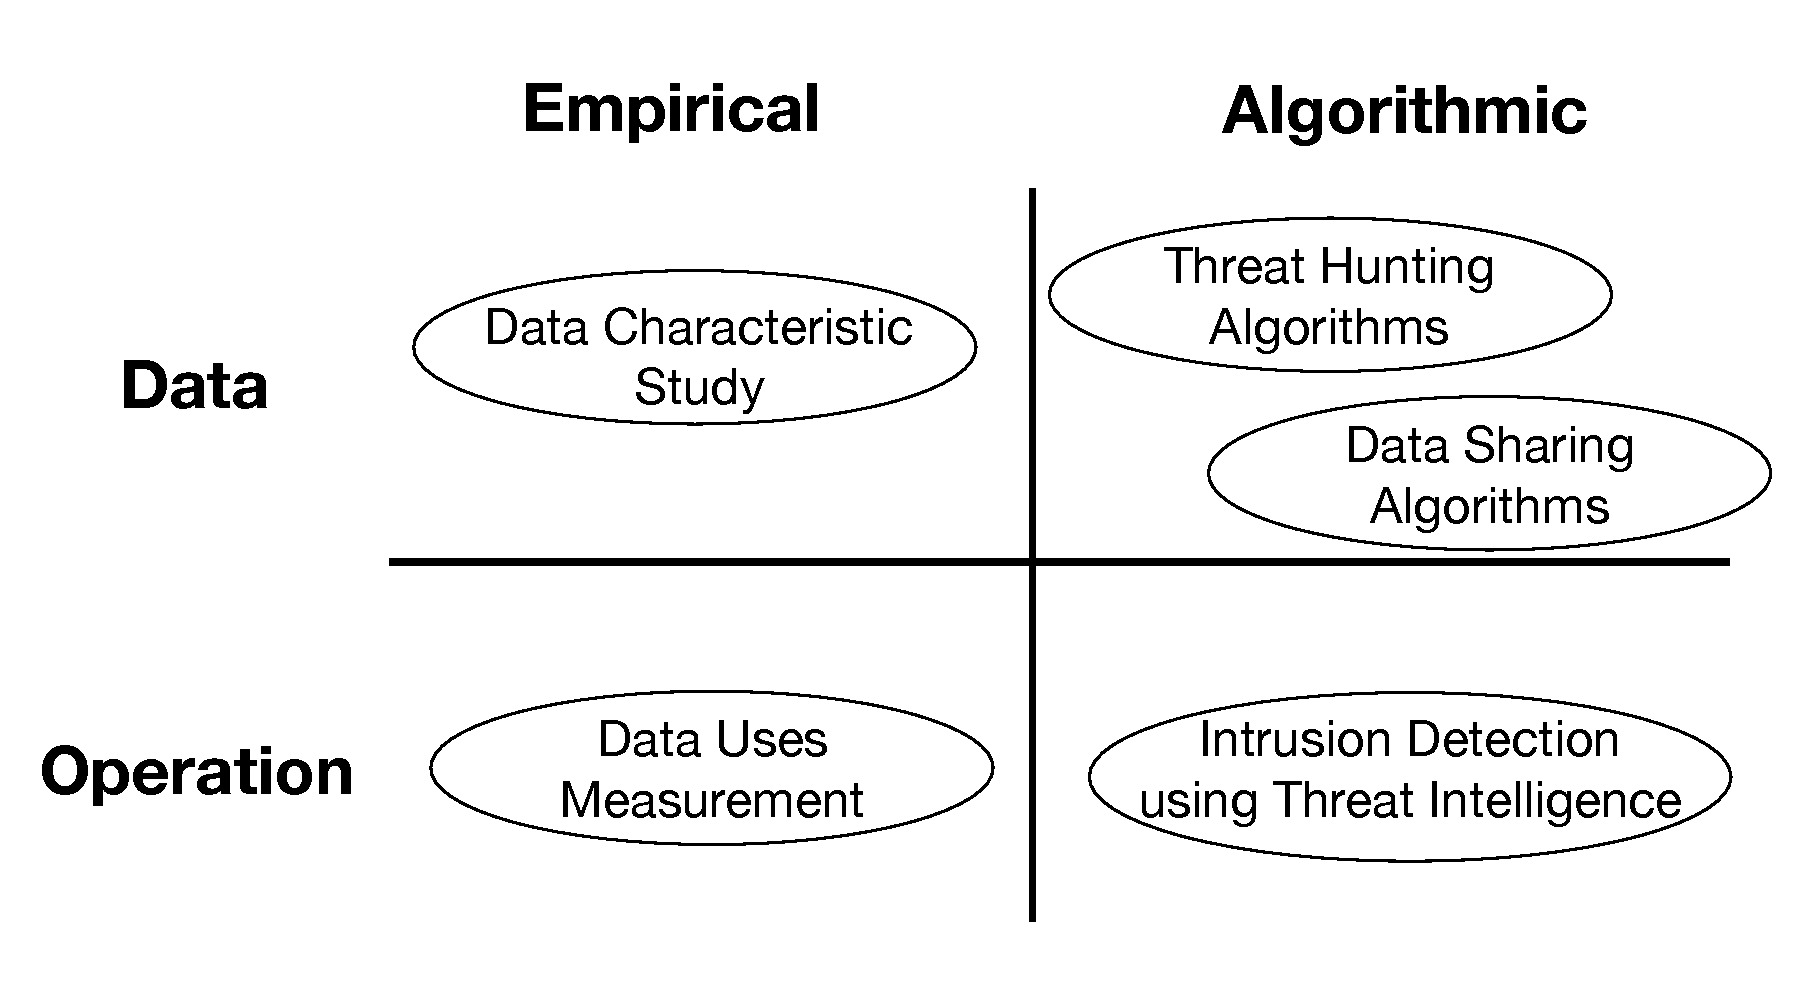
\includegraphics[width=0.8\textwidth]{threat_intel_research_overview.pdf}
\caption{Threat Intelligence research overview and example research
topics in each direction.}
\label{fig:threat_intel_overview}
\end{figure}

Therefore, research directions related to Threat Intelligence can be 
viewed in four general categories, as illustrated in
Figure~\ref{fig:threat_intel_overview}. More specifically, the four 
research directions are: 
\begin{prettylist}
    \item Empirical analysis on Threat Intelligence data: \\
    Understanding the characteristic of Threat Intelligence data, different
    data generation systems and their performance, different threat sharing
    strategies and how are they being used in the real-world, etc.
    
    \item Algorithm exploration related to Threat Intelligence data: \\
    Designing algorithms for threat hunting (Threat Intelligence generation),
    specification for data description and protocols for data sharing, etc.
    
    \item Empirical analysis on Threat Intelligence usage: \\
    Measuring how organizations are using Threat Intelligence, the problems 
    when using these data and the impact on the Internet, etc.
    
    \item Algorithm exploration related to Threat Intelligence usages: \\
    Designing better methods to use threat intelligence during system and 
    network defense(e.g. increasing coverage, reducing false positives),
    explore new ways to use threat intelligence data, such as using the 
    data as machine learning training data, etc.
\end{prettylist}

In this dissertation, I take an empirical approach and explore the 
\textit{Data} and \textit{Operation} problems of Threat Intelligence.
I focus on thoroughly understanding the current status of Threat 
Intelligence and will then discuss my takeaways from these analyses.
In the study of \textit{Data}, which will be discussed in Chapter~\ref{chapter:data_character}, 
I analyzed the data characteristics of existing Threat Intelligence products.
I designed mathematics metrics for Threat Intelligence data evaluation,
and with these metrics, I studied \numipfeeds\ distinct IP address 
data feeds, covering six categories of threats, and \numhashfeeds\ distinct
malware file hash feeds, and measured their data characteristic. Through this
work, I revealed the limitation of existing Threat Intelligence data and 
discussed the potential improvements based on my findings. In the study of
\textit{Operation}, which will be discussed in Chapter~\ref{chapter:data_usage},
I measured how Threat Intelligence data is being used on a large scale. 
I designed a method using IP ID side channel that can measure the 
connectivity between two Internet hosts from a third point. With this 
method, I conducted a large scale Internet measurement over {\reflroughnum} 
U.S. hosts and uncovered their uses of {\blacklistnum} popular public IP
blacklists. I further investigated a broader use of blacklists among the 
hosts, and discovered over 73K hosts has shown blacklist related blocking 
behavior. Together, my work provided an in-depth look into the current
status of Threat Intelligence and augmented the knowledge of our community
on this topic.

%\verb!\mainmatter! macro because it should start on page~1.
%\end{dissertationintroduction}

\section{Overview}
\label{sec:overview}

The threat intelligence data collected for this study was obtained by
subscribing to and pulling from numerous public and private 
intelligence sources. These sources ranged from simple blacklists of 
bad IPs/domains and file hashes, to rich threat intelligence exchanges 
with well labeled and structured data.
I refer each item (\eg IP address or file hash) an \emph{indicator}
(after \emph{indicator of compromise}, the industry term for such data items).

In this section, I enumerate the threat intelligence sources, describe
each source's structure and how I collected it, and then define our
measurement metrics for empirically measuring these sources.  When the
source of the data is public, or when I have an explicit agreement to
identify the provider, I have done so.  However, in other cases, the
data was provided on the condition of anonymity and I restrict
myself to only describe the nature of the provider, but not their
identity.  All of the private data providers were appraised of the
nature of my research, its goals and the methodology that I planned
to employ.


%\pp{Try to use feeds when describing all except FB and TS. I've reworked such
%that feeds -> sources}

\subsection{Data Set and Collection}

I use several sources of \ti\ data for my analysis:

\emphpar{Facebook ThreatExchange (FB)~\cite{FBThreatExchange}}
    This is a closed-community platform that allows hundreds of companies and
    organizations to share and interact with various types of labeled threat data.
    As part of an agreement with Facebook, I collected all its data that it shared broadly.
    In subsequent analyses, sources with
    prefix ``FB'' indicate a unique contributor on the Facebook ThreatExchange.

\emphpar{Paid Feed Aggregator (PA)} This is a commercial paid threat intelligence data aggregation
    platform. It contains data collected from over a hundred other
    threat intelligence sources, public or private, together with its own threat data.
    In subsequent analyses all data sources with prefix ``PA''
    are from unique data sources originating from this aggregator.

\emphpar{\feedetiprep\ Service} This commercial service provides an
    hourly-updated blacklist of known bad IP addresses across different attack categories.

\emphpar{Public Blacklists and Reputation Feeds} I collected indicators from public
    blacklists and reputation data sources, including well-known
    sources such as AlienVault~\cite{Alienvault}, Badips~\cite{Badips}, Abuse.ch~\cite{Abuse-ch}
    and Packetmail~\cite{Packetmail}.

Threat Intelligence indicators include different types of data, such as IP address, malicious file hash, Domain,
URL, etc. In this chapter, I focus the analysis on sources that provide IP addresses and file hashes,
as they are the most prevalent data types in my collection.

I collect data from all sources on an hourly basis. However, both the Facebook
ThreatExchange and the Paid Feed Aggregator change their members and contributions
over time, creating irregular collection periods for several of the sub-data sources.
Similarly, public threat feeds had varying degrees of reliability, resulting in
collection gaps. In this chapter, I use the time window from \veryemph{December 1, 2017}
to \veryemph{July 20, 2018} for most of the analyses, as I have the largest number
of active sources during this period. I eliminated duplicates sources (e.g., sources
we collected individually and also found in the {Paid Aggregator}) and
sub-sources (a source that is a branch of another source). I further break IP
sources into separate categories and treat them as individual feeds, as shown in
Section~\ref{sec:ip-analysis}. This filtering leaves us with \numipfeeds\ IP feeds and
\numhashfeeds\ malware file hash feeds.

The ways each \ti\ source collects data varies, and in some cases
the methodology is unknown. For example, {\feedpacketmail} and {\feedetiprep}
collect threat data themselves via honeypots, analyzing malware, etc. Other
sources, such as {Badips} or the Facebook ThreatExchange, collect their
indicators from general users or organizations---\eg\ entities may be attacked
and submit the indicators to these threat intelligence services. These services
then aggregate the data and report it to their subscribers. Through this level of
aggregation the precise collection methodologies and data
providence can be lost.


\subsection{Data Source Structure}
\label{sec:feed-structure}

\ti\ sources in my corpus structure and present data in different ways.
Part of the challenge in producing cross-dataset metrics is normalizing both
the structure of the data as well as its \emph{meaning}. A major structural
difference that influences my analysis occurs between data sources that
provide data in \emph{snapshots} and data sources that provide \emph{events}.

\emphpar{Snapshot}
Snapshot feeds provide periodic snapshots of a set of indicators. More formally, a
snapshot is a set of indicators that is a function of time. It defines, for a given point in
time, the set of indicators that are members of the data source. Snapshot feeds imply
\emph{state}: at any given time, there is a set of indicators that are \emph{in} the feed.
A typical snapshot source is a published list of IPs periodically updated by its maintainer.
For example, a list of command-and-control IP addresses for a botnet may be published as a
snapshot feed subject to periodic updates.

All feeds of file hashes are snapshots and are \emph{monotonic} in the sense that indicators
are only added, not removed, from the feed. Hashes are a proxy for the file
content, which does not change (malicious file content will not change to benign in the future).

\emphpar{Event}
In contrast, event feeds report newly discovered indicators. More formally, an event source
is a set of indicators that is a function of a time \emph{interval.} For a given time interval,
the source provides a set of indicators that were seen or discovered in that time interval.
Subscribers of these feeds query data by asking for new indicators added in a recent time window.
For example, a user might, once a day, request the set of indicators that appeared
in the last 24 hours.

This structural difference is a major challenge when evaluating feeds comparatively.
I need to normalize the difference to make a fair comparison, especially for IP feeds. From a \ti\
consumer's perspective, an \emph{event} feed does not indicate when an indicator will
expire, so it is up to the consumer to act on the age of indicators. Put another way,
the expiration dates of indicators are decided by how users query the feed:
if a user asks for the indicators seen in the last 30 days
when quering data, then there is an implicit 30-day valid time window for these indicators.

In this chapter, I choose a 30-day valid period for all the indicators I collected from event feeds---the same valid period
used in several snapshot feeds, and also a common query window option offered by event feeds.
I then convert these event feeds into snapshot feeds and evaluate all of them in a unified fashion.


\begin{comment}
Snapshot sources are build on a notion of emph{state}, namely, the current indicators
in the list at a certain moment, as indicators could be added and removed from
the source over time. This type of source mainly apply for IP feeds, as IP data
is time sensitive---a malicious IP address discovered now might not be malicious
in the future. One example of such source is {\feedfeodo}\cite{Feodo}, which records
a list of current Command and Control server IPs of Feodo botnet\cite{Feodo-Tracker}
that a site should block.

Event sources, on the other hand, is ``stateless'', they focus on what have been
discovered recently. One example of this type of source is {\feednothink}\cite{Nothink}.
Upon request, it returns the source IPs they collected that have conducted SSH
brute-force attack in the last day, last week or last year, depending on the specified
query option.

This structural difference doesn't concern file hash feeds, since file hashes are time
insensitive---a malicious file hash won't change to benign in the future. One can
think of all file hash feeds as snapshot feeds where indicators never expire.
\end{comment}

\subsection{Threat Intelligence Metrics}
\label{sec:metrics}

%\note{Should explain why each of these metrics is useful.}
The aim of this work is to develop \emph{threat intelligence metrics} that
allow a \ti\ consumer to compare threat intelligence sources and reason about
their fitness for a particular purpose. To this end, I propose six concrete
metrics: \emph{Volume}, \emph{Differential contribution}, \emph{Exclusive contribution},
\emph{Latency}, \emph{Accuracy} and \emph{Coverage}.

%\noteby{KL}{This needs to be updated to \emph{size} and \emph{rate}.}

\metrics \emphpar{Volume} I define the \emph{volume} of a feed to be the total
number of indicators appearing in a feed over the measurement interval. Volume
is the simplest \ti\ metric and has an established history in prior
work~\cite{jung2004empirical,kuhrer2014paint,
trajectory:oakland11,tasters:imc12,sheng2009empirical,sinha2008shades,thomas2016abuse}.
It is also useful to study the daily \emph{rate} of a feed, which quantifies
the amount of data appearing in a feed on a daily basis.

\emph{Rationale}: To a first approximation, volume captures how much
information a feed provides to the consumer. For a feed without false positives
(see \emph{accuracy} below), and if every indicator has equal value to the
consumer, one would prefer a feed of greater volume to a feed of lesser volume.
Of course, indicators do not all have the same value to consumers: knowing the
IP address of a host probing the entire Internet for decades-old
vulnerabilities is less useful than the address of a scanner targeting
organizations in your sector looking to exploit zero-day vulnerabilities.

\metrics \emphpar{Differential contribution} The \emph{differential
contribution} of one feed with respect to another is the number of indicators
in the first that are not in the second during the same measurement period. We
define differential contribution relative to the size of the first feed, so
that the differential contribution of feed $A$ with respect to feed $B$ is
$\mathrm{Diff}_{A,B} = |A \setminus B|/|A|$. Thus, $\mathrm{Diff}_{A,B}=1$
indicates that the two feeds have no elements in common, and
$\mathrm{Diff}_{A,B} = 0$ indicates that every indicator in $A$ also appears in
$B$. It is sometimes useful to consider the complement
of differential contribution, namely the normalized \emph{intersection} of $A$ in $B$,
given by $\mathrm{Int}_{A,B} = |A \cap B|/|A| = 1-\mathrm{Diff}_{A,B}$.

%(Figure~\ref{fig:overall_heatmap}, in Section~\ref{sec:ip-overlap}, for
%example, shows intersection rather than differential contribution, following the
%Taster's Choice convention.)

\emph{Rationale}: For a consumer, it is often useful to know how many \emph{additional}
indicators a feed offers relative to one or more feeds that the consumer has already.
Thus, if a consumer already has feed $A$ and is considering paying for feed $B$,
then $\mathrm{Diff}_{A,B}$ indicates how many new indicators feed $A$ will provide.

\metrics \emphpar{Exclusive contribution} The \emph{exclusive contribution} of
a feed with respect to a set of other feeds is the proportion of indicators
unique to a feed, that is, the proportion of indicators that occur in the feed
but no others. Formally, the exclusive contribution of feed $A$
is defined as $\mathrm{Uniq}_{A,B} = |A \setminus \bigcup_{B\neq A}B|/|A|$.
Thus, $\mathrm{Uniq}_{A,B} = 0$ means that every element of feed $A$ appears in
some other feeds, while $\mathrm{Uniq}_{A,B}=1$ means no element of $A$ appears
in any other feed.

%Exclusive contribution was first described for domain feeds
%in Taster's Choice~\cite{tasters:imc12}.

\emph{Rationale}: Like differential contribution, exclusive contribution tells
a \ti\ consumer how much of a feed is different. However, exclusive contribution
compares a feed to all other feeds available for comparison, while differential
contribution compares a feed to just another feed. From a \ti\ consumer's
perspective, exclusive contribution is a general measure of a feed's unique
value.
%A feed that aggregates several other feeds may have no exclusive
%contribution, but may provide great value to a consumer.

\metrics \emphpar{Latency} For an indicator that occurs in two or more feeds, its
\emph{latency} in a feed is the elapsed time between its first appearance in any
feed and its appearance in the feed in question. In the feed where an indicator
first appeared, its latency is zero. For all other feeds, the latency indicates
how much later the same indicators appears in those feeds. Taster's
Choice~\cite{tasters:imc12} referred to latency as \emph{relative first appearance
time}. (I find the term \emph{latency} to be more succinct without loss of
clarity.) Since latency is defined for one indicator, for a feed it makes sense
to consider statistics of the distribution of indicator latencies, such as the
median indicator latency.

\emph{Rationale}: Latency characterizes how quickly a feed includes new
threats: the sooner a feed includes a threat, the more effective it is at
helping consumers protect their systems. Indeed, several studies report on the
impact of feed latency on its effectiveness at
thwarting spam~\cite{blacklisting:weis14,ramachandran2007filtering}.

The metrics above are defined without regard for the \emph{meaning} of the
indicators in a feed. One can calculate the volume of a single feed or the
differential contribution of one feed with respect to another regardless of
what the feed purports to contain. While these metrics are easy to compute,
they do little to tell us about the fitness of a feed for a particular purpose.
For this, I need to consider the meaning or purpose of the feed data, as
advertised by the feed provider. I define the following two metrics.

\metrics \emphpar{Accuracy} The \emph{accuracy} of a feed is the proportion of
indicators in a feed that are correctly included in the feed. Feed accuracy is
analogous to \emph{precision} in Information Retrieval. This metric presumes
that the description of the feed is well-defined and describes a set of elements
that should be in the feed given perfect knowledge. In practice, 
researchers have neither
perfect knowledge nor a perfect description of what a feed should contain. In
some cases, however, I can construct a set $A^-$ of elements that should
definitely not be in a feed $A$. Then $\mathrm{Acc}_A \le |A\setminus A^-|/|A|$.

\emph{Rationale}: The accuracy metric tells a \ti\ consumer how many false
positives to expect when using a feed, and, therefore, dictates how a feed
can be used. For example, if a consumer automatically blocks all traffic to
IP addresses appearing in a feed, then false positives may cause disruption
in an enterprise by blocking traffic to legitimate sites. On the other hand,
consumers may tolerate some false positives if a feed is only used to
gain additional insight during an investigation.

\metrics \emphpar{Coverage} The \emph{coverage} of a feed is the proportion
of the intended indicators contained in a feed. Feed coverage is analogous
to \emph{recall} in Information Retrieval. Like accuracy, coverage presumes
that the description of the feed is sufficient to determine which elements
should be in a feed, given perfect knowledge. In some cases, it is possible
to construct a set $A^+$ of elements that should be in a feed. I can then
upper-bound the coverage $\mathrm{Cov}_A \le |A|/|A^+|$.


\emph{Rationale}: For a feed consumer who aims to obtain complete protection
from a specific kind of threat, coverage is a measure of how much protection
a feed will provide. For example, an organization that wants to protect itself
from a particular botnet will want to maximize its coverage of that botnet's
command-and-control servers or infection vectors.

In the following two sections, I use these metrics to evaluate two types of
\ti: IP address feeds and file hash feeds.

\section{IP Threat Intelligence}
\label{sec:ip-analysis}

One of the most common forms of \ti\ are feeds of IP addresses considered malicious,
suspicious, or otherwise untrustworthy. This type of threat intelligence dates back
at least to the early spam and intrusion detection blacklists, many of which are
still active today such as SpamhausSBL~\cite{SpamhausSBL}, CBL~\cite{CBL} and
SORBS~\cite{SORBS}. Here, we apply the metrics described above to quantify the
differences between \numipfeeds\ different IP address \ti\ feeds.
%The overview of the these feeds is summarized in Table~\ref{tab:volume-overview-1}.


\subsection{Feed Categorization}
IP address \ti\ feeds have different meanings, and, therefore, purposes. To
meaningfully compare feeds to each other, we first group feeds into
\emph{categories} of feeds whose indicators have the same intended meaning.
Unfortunately, there is no standard or widely accepted taxonomy of IP \ti\ feeds.
To group feeds into semantic categories, we use metadata associated with the
feed as well as descriptions of the feed provided by the producer, as described below.

\emphpar{Metadata} Some feeds provide category information with each indicator as
metadata. More specifically, all of the {Paid Aggregator} feeds, {\feedalienvault}
and {\feedetiprep} include this category metadata. In this case, we use its pre-assigned
category in the feed. Facebook ThreatExchange feeds do not include category
information in the metadata, but instead provide a descriptive phrase with each indicator.
We then derive its category based on the description.

\emphpar{Feed description} For feeds without metadata, we rely on online descriptions
of each feed, where available, to determine its semantic category. For example, the
website of feed {\feednothink}~\cite{Nothink} describes that the feed reports brute-force
login attempts on its corresponding honeypot, which indicates the feed belongs to
brute-force category.

We grouped our IP feeds into categories derived from the information
above. In this work, we analyze six of the most prominent categories:
%, listed below.
%
\begin{categorylist}\small
\item[Scan] Hosts doing port or vulnerability scans.
\item[Brute-force] Hosts making brute force login attempts.
\item[Malware] Malware C\&C and distribution servers.
\item[Exploit] Hosts trying to remotely exploit vulnerabilities.
\item[Botnet] Compromised hosts belonging to a botnet.
\item[Spam] Hosts that sent spam or should not originate email.
\end{categorylist}
%
Table~\ref{tab:volume-overview-1} lists the feeds, grouped by category, used in the
rest of this section. The symbols \snapfeedsym\ and \deltafeedsym\ before the feed
name indicate whether the feed is a snapshot feed or an event feed, respectively
(see Section~\ref{sec:feed-structure}).
All data was collected during our measurement period,
\veryemph{December 1st, 2017} to \veryemph{July 20th, 2018}. Note that a few
feeds, like {\feedetiprep}, appear in multiple categories. In these feeds, indicators
are associated with different categories via attached metadata. We split these feeds
into multiple virtual feeds each containing indicators belonging to the same category.

\subsection{Volume}
\label{sec:ip-volume}

%\noteby{KL}{Change this to Size and Rate.}
Volume is one of the oldest and simplest \ti\ metrics representing how informative
each data source is. Table~\ref{tab:volume-overview-1} and Table~\ref{tab:volume-overview-2} shows the total number of unique IP addresses
collected from each feed during the measurement period, under column \emph{Volume}. A \snapfeedsym\ denotes a \textit{snapshot feed}
and \deltafeedsym\ indicates an \textit{event feed} (Section~\ref{sec:feed-structure}).
\colname{Volume} is the total number of IPs collected during our measurement period.
\colname{Exclusive} is the exclusive contribution of each feed (Section~\ref{sec:ip-unique}).
\colname{Avg. Rate} is the number of average daily new IPs added in the feed (Section~\ref{sec:ip-accuracy}), and
\colname{Avg. Size} is the average working set size of each feed (Section~\ref{sec:ip-volume}).
Feeds are listed in order of decreasing volume, grouped by category.
The numbers we show are after the removal of invalid entries identified
by the sources themselves. Column \emph{Avg. Rate} shows the average number of
new IPs we received per day, and \emph{Avg. Size} lists the average daily
working set size of each feed, that is, the average size of the snapshot.

\finding\ Feeds vary dramatically in volume. Within every category, big feeds can contain
orders of magnitude more data than small feeds. For example, in the scan category, we saw
over 361,004 unique IP addresses in \feeddshield\ but only 1,572 unique addresses
in \feedTSAnalyst\ in the same time period. Clearly, volume is a major differentiator
for feeds. %In Section~\ref{sec:ip-overlap} and~\ref{sec:ip-unique}, we will examine which
%feeds duplicate each other and which feeds contribute unique indicators.

%\newcolumntype{H}{>{\setbox0=\hbox\bgroup}c<{\egroup}@{}}

\begin{table}[t!]
\centering
\caption{IP \ti\ feeds used in the study part I}
\label{tab:volume-overview-1}
\small
 \begin{tabular}{l@{}r r r r}
 \toprule
 \colname{Feed} & \colname{Volume} & \colname{Exclusive} & \colname{Avg. Rate} &  \colname{Avg. Size} \\ %& \colname{Unrt} \\
  \midrule
  \textbf{Scan Feeds} \\
  %\cline{1-1}

\snapfeedsym\  {\feedTSAlienVault}\footnote{This feed is aggregated by \emph{PA} from Alienvault OTX,
                                            the {\feedalienvault} is the public reputation feed we collected
                                            from AlienVault directly. They are different feeds.}

                                     & 425,967 	& 48.6\% 	& 1,359  & 128,821 \\
\deltafeedsym\ {\feeddshield}        & 361,004 	& 31.1\% 	& 1,556  & 69,526 \\
\snapfeedsym\  {\feedTSramnode}      & 258,719 	& 62.0\% 	& 870    & 78,974 \\
\deltafeedsym\ {\feedpacketmail}     & 246,920 	& 48.6\% 	& 942    & 29,751 \\
\snapfeedsym\  {\feedetiprep}        & 204,491 	& 75.6\% 	& 1,362  & 8,756 \\
\snapfeedsym\  {\feedTSLabScan}      & 169,078 	& 63.1\% 	& 869 	 & 9,775 \\
\snapfeedsym\  {\feedTSSnort}        & 19,085 	& 96.3\% 	& 56     & 4,000 \\
\deltafeedsym\ {\feedFBBasecamp}     & 6,066 	& 71.3\% 	& 24     & 693 \\
\snapfeedsym\  {\feedTSAnalyst}      & 1,572 	& 34.5\% 	& 6.3 	 & 462 \\


  %\midrule
  \textbf{Botnet Feeds} \\
  %\cline{1-1}
\snapfeedsym\  {\feedTSAnalyst}     & 180,034 	& 99.0\% 	& 697 	    & 54,800 \\
\snapfeedsym\  {\feedTSCI}          & 103,281 	& 97.1\% 	& 332 	    & 30,388 \\
\snapfeedsym\  {\feedetiprep}       & 77,600 	& 99.9\% 	& 567 	    & 4,278 \\
\snapfeedsym\  {\feedTSBotscout}    & 23,805 	& 93.8\% 	& 81 	    & 7,180 \\
\snapfeedsym\  {\feedTSVoIP}        & 10,712 	& 88.0\% 	& 40 	    & 3,633 \\
\snapfeedsym\  {\feedTSCompr}       & 7,679 	& 87.0\% 	& 21 	    & 2,392 \\
\snapfeedsym\  {\feedTSBots}        & 4,179 	& 80.7\% 	& 16 	    & 1,160 \\
\snapfeedsym\  {\feedTSHoneypot}    & 2,600 	& 86.5\% 	& 8.5 	    & 812 \\


  %\midrule
  \textbf{Brute-force Feeds} \\
  %\cline{1-1}
\deltafeedsym\  {\feedbadipssh}     & 542,167 	& 84.1\% 	& 2,379 	& 86,677 \\
\deltafeedsym\  {\feedbadipbot}     & 91,553 	& 70.8\% 	& 559 	    & 17,577 \\
\snapfeedsym\   {\feedetiprep}      & 89,671 	& 52.8\% 	& 483 	    & 3,705 \\
\snapfeedsym\   {\feedTSBrute}      & 41,394 	& 92.1\% 	& 138 	    & 14,540 \\
\deltafeedsym\  {\feedusername}     & 37,198 	& 54.2\% 	& 179 	    & 3662.8 \\
\deltafeedsym\  {\feeddisco}        & 31,115 	& 43.6\% 	& 40 	    & 1,224 \\
\deltafeedsym\  {\feedFBZendesk}    & 22,398 	& 77.3\% 	& 74 	    & 2,086 \\
\deltafeedsym\  {\feednothink}      & 20,325 	& 62.7\% 	& 224 	    & 12,577 \\
\deltafeedsym\  {\feeddangerrule}   & 10,142 	& 4.88\% 	& 37	    & 1,102 \\

  %\midrule
  \textbf{Malware Feeds} \\
  %\cline{1-1}
\snapfeedsym\  {\feedetiprep} 	     & 234,470 	& 99.1\% 	& 1,113 	& 22,569 \\
\deltafeedsym\ {\feedFBAdmin} 	     & 30,728 	& 99.9\% 	& 129 	    & 3,873 \\
\snapfeedsym\  {\feedfeodo} 	     & 1,440 	& 47.7\% 	& 1.3 	    & 1,159 \\
\snapfeedsym\  {\feedTSLabMalware}   & 1,184 	& 84.6\% 	& 3.5 	    & 366 \\
\deltafeedsym\ {\feedmalcode} 	     & 865 	    & 61.0\% 	& 2.9 	    & 86.6 \\
\snapfeedsym\  {\feedTSBambenek}     & 785 	    & 92.1\% 	& 3.4 	    & 97.9 \\
\snapfeedsym\  {\feedTSSSL} 	     & 676 	    & 53.9\% 	& 2.9 	    & 84.0 \\
\snapfeedsym\  {\feedTSAnalyst}	     & 492 	    & 79.8\% 	& 2.1 	    & 149 \\
\snapfeedsym\  {\feedTSAbusech}      & 256 	    & 7.03\% 	& 1.6 	    & 117 \\
\snapfeedsym\  {\feedTSMalTraffic}   & 251 	    & 60.5\% 	& 0.9 	    & 72 \\
\snapfeedsym\  {\feedzeus}           & 185 	    & 49.1\% 	& 0.5 	    & 101 \\
\bottomrule
\end{tabular}
\end{table}


\begin{table}[t!]
\centering
\caption{IP \ti\ feeds used in the study part II}
\label{tab:volume-overview-2}
\small
 \begin{tabular}{l@{}r r r r}
 \toprule
 \colname{Feed} & \colname{Volume} & \colname{Exclusive} & \colname{Avg. Rate} &  \colname{Avg. Size} \\ %& \colname{Unrt} \\
  \midrule
  %\midrule
  \textbf{Exploit Feeds} \\

\deltafeedsym\  {\feedbadiphttp}    & 305,020 	& 97.6\% 	& 1,592 	& 22,644 \\
\deltafeedsym\  {\feedbadipftp}     & 285,329 	& 97.5\% 	& 1,313 	& 27,601 \\
\deltafeedsym\  {\feedbadipdns}     & 46,813 	& 99.3\% 	& 231 	& 4,758 \\
\deltafeedsym\  {\feedbadiprfi}     & 3,642 	& 91.4\% 	& 16 	& 104 \\
\deltafeedsym\  {\feedbadipsql}     & 737 	    & 79.5\% 	& 4.4 	& 99.2 \\

 \textbf{Spam Feeds} \\
  %\cline{1-1}
\snapfeedsym\  {\feedetiprep}       & 543,583 	& 99.9\% 	& 3,280 	& 6,551 \\
\deltafeedsym\ {\feedbadippostfix}  & 328,258 	& 90.5\% 	& 842 	    & 27,951 \\
\deltafeedsym\ {\feedbadipspam}     & 302,105 	& 89.3\% 	& 1,454 	& 30,197 \\
\snapfeedsym\  {\feedTSBotscout}    & 14,514 	& 89.3\% 	& 49 	& 4,390 \\
\snapfeedsym\  {\feedalienvault}    & 11,292 	& 96.6\% 	& 48 	& 1,328 \\

\bottomrule
\end{tabular}
\end{table}

%\footnotetext{}



Average daily rate represents the amount of new indicators collected from a feed each day.
Some feeds may have large volume but low daily rates, like {\feedfeodo} in the malware
category. This means most indicators we get from that feed are old data present in the feed before our
measurement started. On the other hand, the average rate of a feed could be
greater than the volume would suggest, like {\feednothink} in the brute-force category.
This is due to the fact that indicators can be added and removed multiple times in a
feed. In general, IP indicators tend to be added in a feed only once: 37 among \numipfeeds\
IP feeds have over 80\% of their indicators appearing only once, and 30 of them have this rate over 90\%.
One reason is that some snapshot feeds maintain a valid period for each indicator, as
we found in all \emph{PA} feeds where the expiration date of each indicator is explicitly
recorded. When the same indicator is discovered again by a feed before its expiration time,
the feed will just extend its expiration date, so this occurrence will not be captured
if we simply subtract the old data from the newly collected data to derive what is added on a day.
For event feeds and snapshot feeds in \emph{PA} where we can precisely track every occurrence
of each indicator, we further examed data occurrence frequency and still found that the vast
majority of IPs in feeds only occurred once---an observation that relates to the dynamics
of cyber threats themselves.

\feednothink, as we mentioned above, is a notable exception. It has over 64\% of its
indicators appearing 7 times in our data set. After investigating, we
found that this feed posts all its previous data at the end of every month, behavior very likely
due to the feed provider instead of the underlying threats.
% {\feedusername}, {\feedbadipftp}, {\feedbadipdns} and {\feedbadipsql}
% all have a large percent of IPs appeared twice, and we found
% that all 4 feeds reported a abnormally large amount of same IPs on 2018 July 1st and July 13th.
% We will discuss more about this in Section~\ref{sec:ip-accuracy}.

The working set size defines the daily average amount of indicators users need to store in their
system to use a feed (the storage cost of using a feed). The average
working set size is largely decided by the valid period length
of the indicators, controlled either
by the feed (snapshot feeds) or the user (event feeds). The longer the valid period is,
the larger the working set will be. Different snapshoot feeds have different choices for this
valid period: {\feedTSAlienVault} in the scan category sets a 90-day valid period for
every indicator added to the feed, while {\feedTSAbusech} uses a 30-day period. Although we do not
know the data expiration mechanism used by snapshot feeds other than \emph{PA} feeds, as
there is no related information recorded, we can still roughly estimate this by checking the
\emph{durations} of their indicators---the time between an indicator being added and being removed.
Four {\feedetiprep} feeds have more than 85\% of durations shorter than 10 days, while the one in
the malware category has more than 40\% that span longer than 20 days. {\feedfeodo} has over 99\% of
its indicators valid for our entire measurement period, while over 70\% of durations in the
{\feedzeus} are less than 6 days. We did not observe a clear pattern regarding how each snapshot
feed handles the expiration of indicators.

%The column \emph{Occurred} presents the number of unique IPs added in a \ti\ source after our
%measurement period started. We differentiate \emph{Volume} and \emph{Occurred} since IP
%indicators are time sensitive: They are added, removed and could be added again in a feed over
%time. When we pull data from a snapshot feed on a day, some IPs are actually added
%on previous days and are still kept by the feed. \emph{Occurred} only captures the IPs that
%are newly added after the measurement period started, while \emph{Volume} includes legacy data in
%a feed when we collect indicators on the first day of our analysis. At a high level,
%\emph{Volume} represents the number of IPs that a feed \emph{considers} as malicious during
%a period of time, and \emph{Occurred} represents the number of newly discovered indicators by the
%feed during that time.

%For delta feeds, we calculated their \emph{Volume} by tracking the expiration dates of the
%indicators we collected before (The expiration dates are provided in the metadata) and included
%the indicators whose expiration dates are after January 1st, 2016.

\subsection{Differential Contribution and Intersection}
\label{sec:ip-overlap}

%It is often useful to know whether a potential new feed contributes any new indicators relative to what a \ti\ consumer has already.
The differential contribution metric measures the number of indicators in one feed that are not in another. Equivalently, we can consider the intersection of two feeds, which is the number of elements in one feed that are present in the other, normalized by the size of the first: $|A\cap B|/|A|$. Figure~\ref{fig:overall_heatmap} shows the intersection relationship of all feeds in the study. Each cell in the matrix represents the number of elements in both feeds, normalized by the size of the feed spanning the rows on the table. That is, $A$, in the expression above, ranges over rows, and $B$ over columns of the matrix. Darker (more saturated) colors indicate greater intersection. Comparisons of feeds within a category are shaded red and comparisons of feeds between different categories are shaded blue. Note that the matrix is asymmetric, because, in general, $|A\cap B|/|A| \neq |A\cap B|/|B|$. Elements of the matrix are in the same order as in Table~\ref{tab:volume-overview-1}.

\begin{figure}
\centering
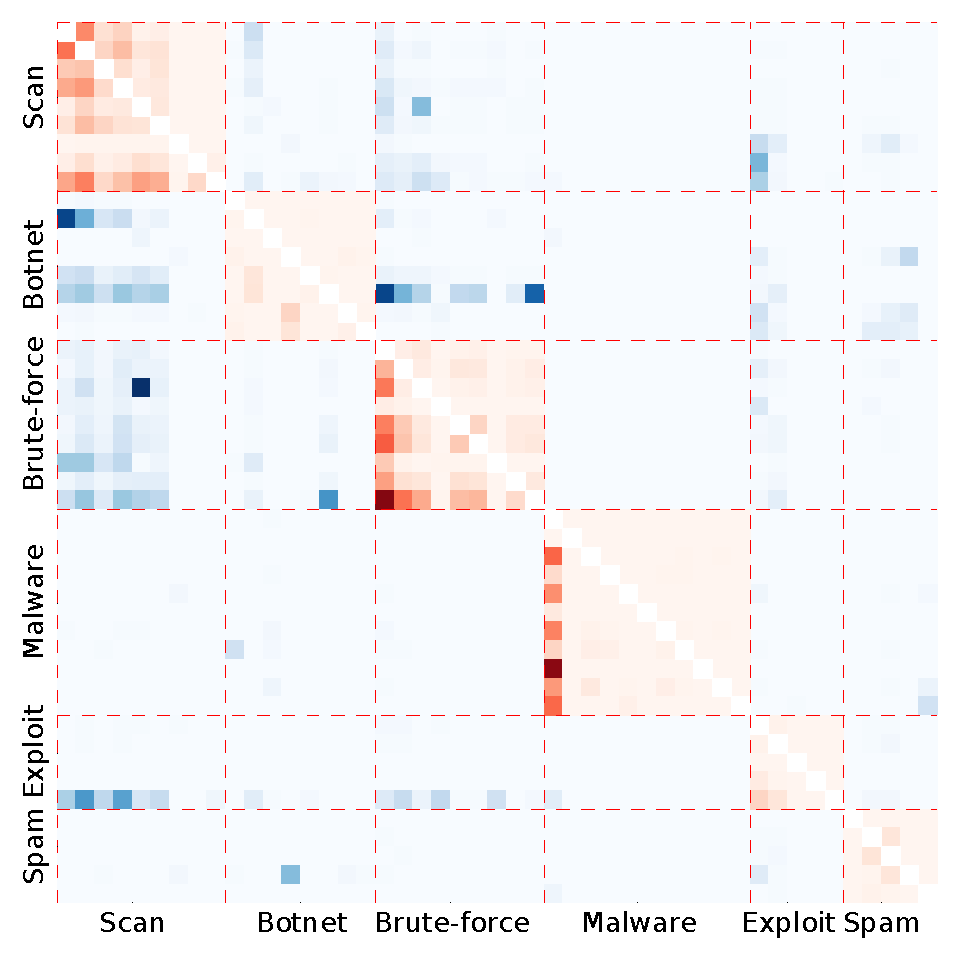
\includegraphics[width=0.475\textwidth]{images/overall_heatmap.pdf}
\caption{Feed intersection for all IP feeds. Each row/column represents a feed, shown in the same order as Table~\ref{tab:volume-overview-1}. Darker (more saturated) colors indicate greater intersection.}
\label{fig:overall_heatmap}
\end{figure}

%\begin{figure}
%\centering
%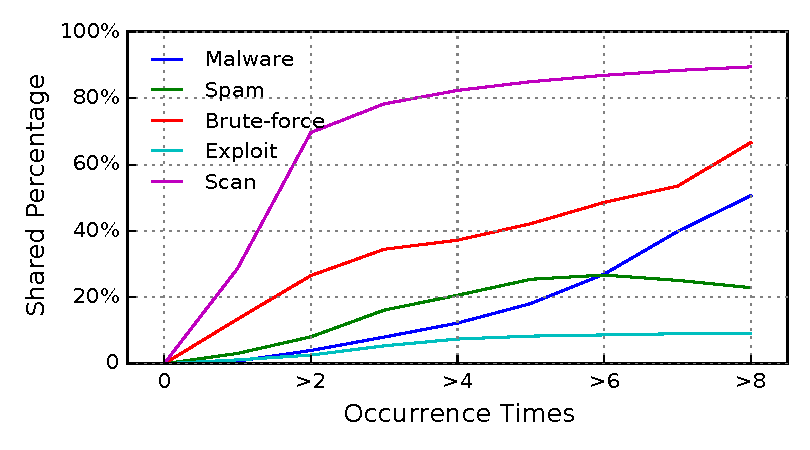
\includegraphics[width=0.4\textwidth]{images/occur_vs_overlap.pdf}
%\caption{Relation between indicators' occurrence frequency and the percentage of being shared. Each point on a line means: For the %indicators that had occurred >\emph{x} times in a feed(\textbf{X} axis), how much percent of them are shared among at least two feeds within its category(\textbf{Y} axis).}
%\label{fig:occur_vs_overlap}
%\end{figure}

\finding\ Feeds in scan and brute-force categories have higher pairwise intersections: Half of the pairwise intersection rates in two categories are greater than 5\%. The scan category has 29 out of 72 pairs (excluding self comparisons) with an intersection rate larger than 10\%, and the same case occurred in 19 out of 72 pairs in the brute-force category.

On the other side, feeds in the botnet, exploit, malware and spam category do not share much data between each other: all 4 categories have more than three-quarters of pairwise intersection rates less than 1\%. A few big feeds in these categories can share a significant amount of data with some small feeds in the same category---a characteristic that appears as a dark vertical line within its category in Figure~\ref{fig:overall_heatmap}. \feedetiprep\ in the malware category, for example, shares over 30\% of 6 other malware feeds. But the intersections among the vast majority of feeds in these 4 categories are low. This finding is consistent with prior work~\cite{metcalf2015blacklist,thomas2016abuse}, but we provide a more comprehensive view regarding different categories.

Figure~\ref{fig:overall_heatmap} also shows the relation between feeds across different categories. We can clearly see a relation between scan and brute-force feeds: multiple scan feeds have non-trivial intersection with feeds in the brute-force category. In fact, 23.1\% of all 760,263 brute-force IPs we collected are also included by scan feeds in our dataset. There are also three botnet feeds---\feedTSCI, \feedTSVoIP\ and \feedTSCompr---that have over 10\% of its data shared with multiple feeds in the scan category.

%\noteby{KL}{Cut this paragraph and accompanying figure.}
%One interesting question is: Are indicators that occurred multiple times in a feed more likely to be shared between feeds? We check this question by calculating how much percent of indicators, that had occurred more than \emph{x} times in a feed, are shared between at least two feeds within each category. The result is shown in Figure~\ref{fig:occur_vs_overlap}. Botnet category is excluded from the Figure since the percentages are too low to argue about the trend. We can see that there is a strong positive correlation between the occurrence frequency and the percentage being shared, across different categories. This aligns with the intuition that a persistent attacker is more likely being observed by mulitple \ti\ sources.

\subsection{Exclusive Contribution}
\label{sec:ip-unique}

Exclusive contribution represents the number of indicators in a feed that are in no other feeds. I calculate each feed's exclusive contribution among all the feeds in the same category, emphasizing their uniqueness regarding the scope of data they claim to report. Each feed's exclusive contribution is presented in Table~\ref{tab:volume-overview-1} in column \emph{Exclusive}, calculated based on its volume.

\finding\ As I already observed in Section~\ref{sec:ip-overlap}, botnet, exploit and spam feeds have relatively low pairwise intersections. Consequently, the feeds in these four categories have high exclusive contribution rates in general: the median exclusive contribution rates of these four categories are 90.9\%, 97.5\% and 90.5\%, respectively. The malware category has a low median exclusive rate, since multiple small feeds have non-trivial intersection with the largest feed {\feedetiprep}, but the two largest feeds in malware both have a exclusive rate over 99\%. Scan and brute-force feeds have more intersection within its category, and their exclusive rates are lower: 62.0\% median rate in scan and 62.7\% in brute-force, and the top two largest feeds in both categories have an exclusive rate below 85\%.

If one assumes a process where a feed is more likely to have popular elements, then smaller feeds would be subsumed by larger feeds. Yet, for some small feeds like {\feedmalcode} in the malware and {\feedTSHoneypot} in the botnet categories, even though they are several orders of magnitude smaller than the largest feeds in their categories, a significant proportion of their indicators is still unique to the feed. When I aggregate the data in each category, 73\% of all scan feed indicators are unique to a single feed and 88\% of brute force feed indicators are unique to one feed. For other categories, over 97\% of elements in the category are unique to a single feed. This result agrees with previous work that most data in threat intelligence feeds is unique~\cite{metcalf2015blacklist,thomas2016abuse}.
\subsection{Latency}
\label{sec:ip-timing}

% Data Occurrence analysis
Feed latency measures how quickly a feed reports new threat indicators. The
sooner a feed can report potential threats, the more valuable it is for
consumers. The absolute latency of an indicator in a feed is the time from
the beginning of the corresponding event until when the indicator shows up in
the feed. However, it is difficult to know the actual time when an event begins
from the threat intelligence data. Instead, we measure the \textit{relative
latency}, which is the delay of an indicator in one feed to be the time between
its appearance in that feed and the first seen among all the feeds.

\begin{figure}[t!]
\centering
\subfloat[Latency distribution in scan feeds]{
	\label{fig:scan_firstseen}
	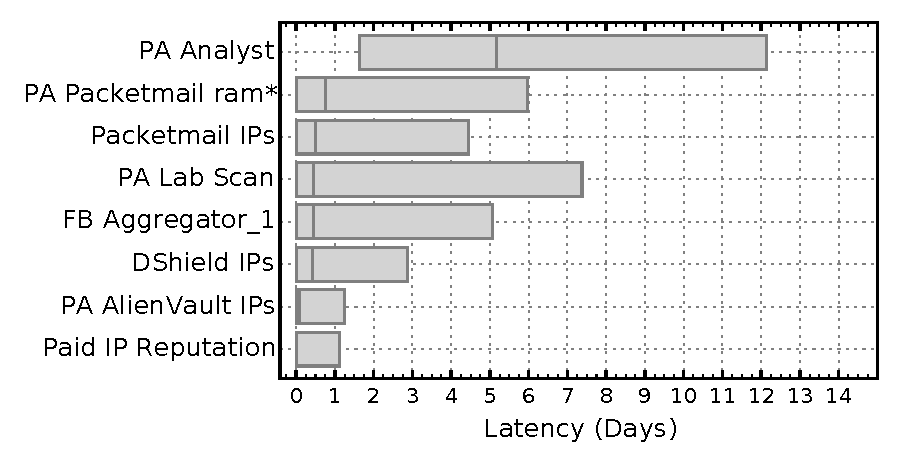
\includegraphics[width=0.8\textwidth]{data_character/images/scan_latency_new.pdf}}

\subfloat[Latency distribution in brute-force feeds]{
	\label{fig:brute_firstseen}
	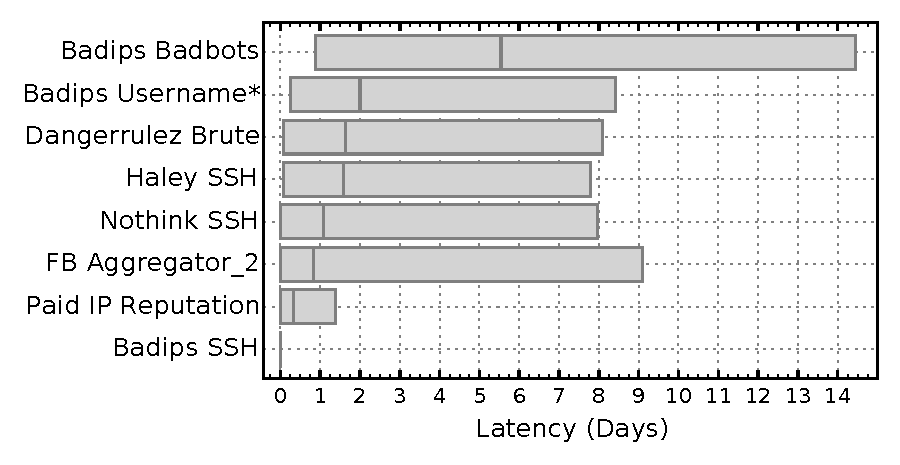
\includegraphics[width=0.8\textwidth]{data_character/images/brute_latency_new.pdf}}

\caption{Distribution of indicators' latency in scan and brute-force feeds.}
\label{fig:firstseen}
\end{figure}


Relative latency can only be calculated for
indicators that occur in at least two feeds. As discussed in
Section~\ref{sec:ip-unique}, the number of common indicators in the botnet, malware, exploit and spam feeds is very low (fewer than 3\% of elements occur in more than one feed). Relative latency calculated for these feeds is less meaningful. For this analysis, therefore, we focus on scan and brute-force feeds.

Another issue is the time sensitivity of IP threats. An event that originated from
an IP address, like scanning activity or a brute-force attack, will not last
forever. If one scan feed reports an IP address today and another feed reports
the same IP three months later, it would make little sense to consider them as one
scanning event and label the second occurrence as being three months late.
Unfortunately, there is no easy way we can clearly distinguish events from each
other. Here we use a one-month window to restrict an event, assuming that the same
attack from one source will not last for more than 30 days; although arbitrary, it provides a reasonably conservative threshold, and experimenting with other thresholds produced similar overall results. More specifically, we calculate relative latency by tracking the
first occurrence of IPs in all feeds in a category, then recording the latency of the
following occurrences while excluding ones that occur after 30 days. By just
using the first appearance of each IP as the base, we avoid the uncertainty caused by
multiple occurrence of indicators and different valid periods used among feeds.

%We also used other time windows for the latency calculation and the results are very similar.

Figures~\ref{fig:scan_firstseen} and~\ref{fig:brute_firstseen} show the relative
latency distribution among feeds in the scan and brute-force categories, in hours. Each box shows the latency distribution of shared IPs in the feed calculated in hours
from 25 percentile to 75 percentile, with the middle line indicating the median.
(``Badips Username*'' here is the abbreviation for feed name Badips
Username Notfound; ``PA Packetmail Ram*'' for PA Packetmail Ramnode)
We focus on just those feeds that have
over 10\% of their data shared with others to ensure the analysis can represent the latency
distribution of the overall feed. There is one feed in each category ({\feedTSSnort}
in scan and {\feedTSBrute} in brute-force) that is excluded from the figure.

\finding\
From the distribution boxes we can see that {\feedetiprep} in scan and {\feedbadipssh}
in brute-force are the fastest feeds in their category, as they have the lowest median
and 75th percentile latencies. On the other hand, {\feedTSAnalyst} in scan and
{\feedbadipbot} in brute-force are the slowest feeds. Figure~\ref{fig:scan_firstseen}
shows that all scan feeds except one have their 25th percentile latency equal to 0, indicating
these feeds, across different sizes, all reported a significant portion of their shared
data first. A similar case also happens in the brute-force category.

%This means that feeds can scan feeds, no matter fast or slow,

One may reasonably ask whether large feeds report data sooner than small feeds.
The result shows that this is not always the case. {\feedFBBasecamp} is the second smallest
feed in our scan category, yet it is no slower than several other feeds which have over 10 times of its daily rate.
{\feedbadipbot}, on the other hand, has the second largest rate in brute-force
category, but it is slower than all the other feeds in the brute-force category. Feeds that are small in volume can still report a lot of their data first.

% This shows that when choosing a feed, we cannot assume its latency by just looking at its volume.

Another factor that could affect latency is whether feeds copy data from each other. For example, 93\% of {\feeddangerrule} also appears in {\feedbadipssh}. If this is the case, we expect {\feeddangerrule} will be faster than {\feedbadipssh} on
reporting their shared data. However, we compared the relative latency between just two feeds and found {\feedbadipssh} reported 88\% of their shared indicators first.
We further conducted this pairwise latency comparison between all feeds in scan, brute-force
and malware (since {\feedetiprep} shares non-trivial amount of data with a
few small feeds in the malware category), and did not see a clear latency advantage between
any two feeds. Note that this observation does \emph{not} prove there is no data
copying, since the shared data between two feeds might partially come from copying and partially from the feeds' own data collection. Furthermore, our latency analysis is at a one-hour granularity.
% We did not find the evidence in latency to prove that there is indeed data copying.

\subsection{Accuracy}
\label{sec:ip-accuracy}
\newcolumntype{H}{>{\setbox0=\hbox\bgroup}c<{\egroup}@{}}

\begin{table}[t!]
\centering
\caption{IP \ti\ feeds accuracy overview. \colname{Unrt} is fraction of unroutable addresses in each feed (Section~\ref{sec:ip-accuracy}).
\colname{Alexa Top} is the number of IPs intersected with top Alexa domain IP addresses, and
\colname{CDNs} is the number of IPs intersected with top CDN provider IP addresses.}
\label{tab:accuracy-overview-1}
\scriptsize
 \begin{tabular}{l r r r r}
 \toprule
 \colname{Feed} & \colname{Added} & \colname{Unrt} & \colname{Alexa} &  \colname{CDNs} \\ %& \colname{Unrt} \\
  \midrule
  \textbf{Scan Feeds} \\
  %\cline{1-1}
{\feedTSAlienVault}  & 313,175 	& 0.0\% 	& 1  & 0 \\
{\feeddshield}       & 339,805 	& 0.03\% 	& 68 & 62\\
{\feedTSramnode}     & 200,568 	& <0.01\% 	& 0  & 0 \\
{\feedpacketmail}    & 211,081 	& 0.0\% 	& 0  & 0 \\
{\feedetiprep}       & 200,915 	& 1.65\% 	& 6  & 21\\
{\feedTSLabScan}     & 169,037 	& <0.01\% 	& 0  & 0 \\
{\feedTSSnort}       & 12,957 	& 0.42\% 	& 1  & 0 \\
{\feedFBBasecamp}    & 5,601 	& 0.0\% 	& 0  & 0 \\
{\feedTSAnalyst}     & 1,451 	& 0.41\% 	& 0  & 0 \\


  %\midrule
  \textbf{Botnet Feeds} \\
  %\cline{1-1}
{\feedTSAnalyst}     & 180,034 	& <0.01\% 	& 0  & 0 \\
{\feedTSCI}          & 76,125 	& <0.01\% 	& 0  & 0 \\
{\feedetiprep}       & 73,710 	& 1.66\% 	& 6  & 74\\
{\feedTSBotscout}    & 18,638 	& 0.09\% 	& 1  & 0 \\
{\feedTSVoIP}        & 9,290   	& 0.32\% 	& 0  & 0 \\
{\feedTSCompr}       & 4,883 	    & 0.0\% 	& 0  & 0 \\
{\feedTSBots}        & 3,594 	    & 0.0\% 	& 0  & 0 \\
{\feedTSHoneypot}    & 1,947 	    & 0.0\% 	& 0  & 0 \\


  %\midrule
  \textbf{Brute-force Feeds} \\
  %\cline{1-1}
{\feedbadipssh}     & 456,605 	& 0.19\% 	& 217  & 1\\
{\feedbadipbot}     & 91,553 	& 1.04\% 	& 46   & 1,251\\
{\feedetiprep}      & 87,524 	& 0.03\% 	& 0  & 10\\
{\feedTSBrute}      & 31,555 	& 0.0\% 	& 0  & 0\\
{\feedusername}     & 37,198 	& 0.53\% 	& 4  & 0\\
{\feeddisco}        & 8,784 	& 0.03\% 	& 0  & 0\\
{\feedFBZendesk}    & 17,779 	& 0.0\% 	& 0  & 0\\
{\feednothink}      & 20,325 	& 1.51\% 	& 2  & 0\\
{\feeddangerrule}   & 8,247 	& 0.0\% 	& 0  & 0\\


  %\midrule
  \textbf{Malware Feeds} \\
  %\cline{1-1}

{\feedetiprep}       & 217,073 	& 0.13\% 	& 291  & 3,489\\
{\feedFBAdmin}       & 29,840 	& 2.14\% 	& 2    & 0\\
{\feedfeodo}         & 296 	& 0.0\% 	& 0   & 0\\
{\feedTSLabMalware}  & 806 	& 2.85\% 	& 0   & 0\\
{\feedmalcode}       & 668 	& 0.0\% 	& 8   & 11\\
{\feedTSBambenek}    & 777 	& 9.13\% 	& 0   & 0\\
{\feedTSSSL}         & 674 	& 0.0\% 	& 0   & 0\\
{\feedTSAnalyst}     & 486 	& 0.0\% 	& 0   & 0\\
{\feedTSAbusech}     & 256 	& 3.12\% 	& 0   & 0\\
{\feedTSMalTraffic}  & 193 	& 0.51\% 	& 0   & 0\\
{\feedzeus}          & 67 	& 0.0\% 	& 1   & 0\\

  %\midrule
  \textbf{Exploit Feeds} \\
{\feedbadiphttp}    & 305,020 	& 0.67\% 	& 16  & 2,590\\
{\feedbadipftp}     & 285,329 	& 1.33\% 	& 14  & 2\\
{\feedbadipdns}     & 46,813 	& 0.50\% 	& 119 & 244 \\
{\feedbadiprfi}     & 3,642 	& 2.22\% 	& 0   & 0\\
{\feedbadipsql}     & 737 	& 1.89\% 	& 0   & 1\\

  \textbf{Spam Feeds} \\
  %\cline{1-1}
{\feedetiprep}      & 543,546 	& 78.7\% 	& 1	& 0 \\
{\feedbadipspam}    & 302,105 	& 0.02\% 	& 19	& 0 \\
{\feedbadippostfix} & 193,674 	& 1.29\% 	& 18	& 1 \\
{\feedTSBotscout}   & 11,358 	& 0.06\% 	& 0  	& 0 \\
{\feedalienvault}   & 10,414 	& 0.07\% 	& 63	& 1,040 \\

\bottomrule
\end{tabular}
\end{table}

%\footnotetext{}


Accuracy measures the rate of false positives in a feed. A false
positive is an indicator that data is labeled with a category to which
it does not belong.  For example, an IP address found in a scan feed
that has not conducted any Internet scanning is one such false
positive.  As well, even if a given IP is in fact associated with
malicious activity, if it is not unambiguously actionable (e.g.,
Google's DNS at 8.8.8.8 is used by malicious and benign software
alike) then for many use cases it must also be treated as a false
positive.  False positives are problematic for a variety of reasons,
but particularly because they can have adverse operational
consequences.  For example, one might reasonably desire to block all
new network connections to and from IP addresses reported as hosting
malicious activity (indeed, this use is one of the promises of threat
intelligence). False positives in such feeds, though, could lead to
blocking legitimate connections as well.  Thus, the degree of accuracy
for a feed may preclude certain use cases.

Unfortunately, determining which IPs belong in a feed and which do not
can be extremely challenging. In fact, at any reasonable scale, I am
unaware of any method for unambiguously and comprehensively
establishing ``ground truth'' on this matter.  Instead, in this
section I report on a proxy for accuracy that provides a
conservative assessment of this question.  To wit, I assemble a
\emph{whitelist} of IP addresses that either should not reasonably be
included in a feed, or that, if included, would cause significant
disruption. The presence of such IPs in a feed are
clearly false positives and thus define an upper bound on a feed's
accuracy.  I populate my list from three sources: unroutable IPs,
IPs associated with top Alexa domains, and IPs of major content
distribution networks (CDNs). The detail result for the accuracy analysis 
is presented in Table~\ref{tab:accuracy-overview-1} and 
Table~\ref{tab:accuracy-overview-2}.
\colname{Unrt} is fraction of unroutable addresses in each feed
(Section~\ref{sec:ip-accuracy}).
\colname{Alexa Top} is the number of IPs intersected with top Alexa domain 
IP addresses, and \colname{CDNs} is the number of IPs intersected with 
top CDN provider IP addresses. I will explain more about each column in below.

\noindent\textbf{Unroutable IPs.} Unroutable IPs are IP addresses that
were not BGP-routable \emph{when they first appeared} in a feed, as
established by contemporaneous data in the RouteViews
service~\cite{Routeview}. While such IPs could have appeared in the
source address field of a packet (i.e., due to address spoofing), it
would not be possible to complete a TCP handshake. Feeds that imply
that such an interaction took place should not include such IPs. For
example, feeds in the Brute-force category imply that the IPs they
contain were involved in brute-force login attempts, but this could
not have taken place if the IPs are not routable. While including
unroutable addresses in a feed is not, in itself, a problem, their
inclusion suggests a quality control issue with the feed, casting
shade on the validity of other indicators in the feed.

To allow for some delays in the feed, I check if an IP was routable
at any time in the seven days prior to its first appearance in a feed,
and if it had, I do not count it as
unroutable. Table~\ref{tab:accuracy-overview-1}, column \textit{Unrt},
shows the fraction of IP indicators that were not routable at any time
in the seven days prior to appearing in the feed. This analysis is
only conducted for the IPs that are added after my measurement
started. The number of such IPs is shown in column \textit{Added}, and
the unroutable fraction shown in \textit{Unrt} is with respect to this
number.

\noindent\textbf{Alexa.} Blocking access to popular Internet sites or
triggering alarms any time such sites are accessed would be disruptive
to an enterprise. For my analysis, I periodically collected the
Alexa top 25 thousand domains (3--4 times a month) over the course of
the measurement period~\cite{alexa}. To address the challenge that
such lists can have significant churn~\cite{scheitle2018long}, we
restrict my whitelist to hold the \emph{intersection} of all these
top 25K lists (i.e., domains that were in the top 25K every time we
polled Alexa over the 8-month measurement period), which left us with
12,009 domains. I then queried DNS for the A records, NS
records and MX records of each domain, and collected the corresponding
IP addresses. In total, I collected 42,436 IP addresses associated
with these domains. I compute the intersection of these IPs
with \ti\ feeds and show the results in column \textit{Alexa} in
Table~\ref{tab:accuracy-overview-1}.


\noindent\textbf{CDNs.} CDN providers serve hundreds of thousands of
sites. Although these CDN services can (and are) abused to conduct
malicious activities~\cite{cdnabuse}, their IP addresses are not
actionable.  Because these are fundamentally shared services,
blocking such IP addresses will also disrupt access to benign
sites served by these IPs.  I collected the IP ranges used by 5
popular CDN providers: AWS CloudFron~\cite{cloudfront},
Cloudflare~\cite{cloudflare}, Fastly~\cite{fastly},
EdgeCast~\cite{edgecast} and MaxCDN~\cite{maxcdn}. I then check how
many IPs in \ti\ feeds fall into these ranges. Column \textit{CDNs} in
Table~\ref{tab:accuracy-overview-1} shows the result.

\finding\ Among the \numipfeeds\ feeds in the table, 33 feeds have at
least one unroutable IP, and for 13 of them, over 1\% of the addresses
they contain are unrouteable. Notably, the {\feedetiprep} feed in the
spam category has an unroutable rate over 78\%.  Although it is not
documented, a likely explanation is that this feed may include unroutable
IPs intentionally, as this is a known practice among certain spam
feeds. For example, the Spamhaus DROP List~\cite{Spamhaus} includes IP
address ranges known to be owned or operated by malicious actors,
whether currently advertised or not. Thus, for feeds that explicitly
do include unroutable IPs, their presence in the feeds should not
necessarily be interpreted as a problem with quality control.

I further checked feeds for the presence of any ``reserved IPs''
which, as documented in RFC 8190, are not globally routable (e.g., private
address ranges, test networks, loopback and multicast).  Indeed,
12 feeds reported at least one reserved IP, including four of the
{\feedetiprep} feeds (excepting the spam category), six of the Badips
feeds, and the {\feedFBAdmin} and {\feeddshield} feeds. Worse, the
{\feedetiprep} feeds together reported over 100 reserved IPs. Since
such addresses should never appear on a public network,
reporting such IPs indicates that a feed provider fails to
incorporate some basic sanity checks on its data.

There are 21 feeds that include IPs from top Alexa domains, as shown
in column \textit{Alexa} in Table~\ref{tab:accuracy-overview-1}. Among
these IPs there are 533 A records, 333 IPs of MX records and 63 IPs of
NS records.  The overlapped IPs include multiple instances from
notable domains. For example, the IP addresses of www.github.com are
included by {\feedmalcode}.  {\feedetiprep} in the malware category
contains the IP address for www.dropbox.com.  {\feedalienvault}
contains the MX record of groupon.com, and {\feedbadipssh} also
contains the IP addresses of popular websites such as www.bing.com.

Most of the feeds I evaluated do not contain IPs in CDN ranges, yet
there are a few (including multiple {\feedetiprep} feeds, Badips feeds
and {\feedalienvault}) that have significant intersection with CDN
IPs. {\feedalienvault} and Badips feeds primarily intersect with
%IPs from
Cloudflare CDN, while most of the overlap in the {\feedetiprep} malware
category overlaps with AWS CloudFront.

Overall, the rate of false positives in a feed is not strongly
correlated with its volume.  Moreover, certain classes of false
positives (e.g., the presence of Top Alex IPs or CDN IPs) seem to
be byproducts of how distinct feeds are collected (e.g., Badips
feeds tend to contain such IPs, irrespective of volume).
Unsurprisingly, I also could find not correlation between a feed's
latency and its accuracy.
\subsection{Coverage}
\label{sec:completeness}

The coverage metric provides a quantitative measure of how well a
feed captures the intended threat. A feed with perfect
coverage would include all indicators that belong in a category.
Unfortunately, as discussed above, there is no systematic way for
evaluating the exact accuracy or coverage of a feed since it is unrealistic
to obtain ground truth of all threat activities on the Internet.

However, there are some large-scale threat activities that are
well-collected and well-studied. One example is Internet
scanning. Researchers have long been using ``Internet telescopes'' to
observe and measure network scanning
activities~\cite{benson2015leveraging, durumeric2014internet,
  pang2004characteristics}.  With a large telescope and well-defined
scan filtering logic, one can obtain a comprehensive view of global
scanning activities on the Internet.

To this end, we collected three months of traffic (from January 1st to
March 31st 2018) using the UCSD network telescope~\cite{telescope},
which monitors a largely quiescent /8 network comprising over 16
million IP addresses.  We then used the default parameters of the Bro
IDS~\cite{BroNetwork} to identify likely scanning traffic, namely
flows in which the same source IP address is used to contact 25 unique
destination IP addresses on the same destination port/protocol within
5 minutes. Given the large number of addressed being monitored, any
indiscriminate scanner observed by \ti\ feeds will likely also be seen
in our data.  Indeed, by intersecting against this telescope data we
are able to partially quantify the coverage of each \ti\ scanning feed.


%(u'TS Alien Vault OTX Malicious IPs', 'scan') 0.966922702159 0.0045119148556
%(u'dshield-ips', 'scan') 0.951590802754 0.00826350821018
%(u'TS Packetmail iprep ramnode', 'scan') 0.933286248198 0.00306798601481
%(u'packetmail-ip', 'scan') 0.87635529608 0.00365935255666
%(u'et-ip-reputation', 'scan') 0.627009603999 0.00230524603455
%(u'TS Anomali Labs MHN', 'scan') 0.855805914736 0.0032333616247
%(u'TS Snort IP BlockList', 'scan') 0.0862598022503 1.2237504915e-05
%(u'FB Basecamp Streetcred', 'scan') 0.153300600109 1.3591853285e-05
%(u'TS Analyst', 'scan') 0.523206751055 1.19956569917e-05

The scanners we collected from the telescope consist of 20,674,149 IP addresses.
The total number of IPs in all the scan feeds during this period is
425,286, which covers only 1.7\% (363,799 shared IPs) of all the telescope scan IPs.
On the other hand, telescope scanners intersect with 85\% of all IPs in scan feeds.
When looking at each feed, {\feedTSAlienVault}, {\feeddshield}
{\feedpacketmail}, {\feedTSLabScan} and {\feedTSramnode} all have over 85\% of their
data intersected with telescope scanners; the other four, though, have less than 65\%
of their data shared (and the rate for {\feedTSSnort} is only 8\%).


To further understand how well each scan feed detects scanning
activities, we measure how different sizes of scanners in the
telescope are covered by each feed. Here, \emph{scanner size} means how
many IPs a scanner has scanned in the telescope within a
day. Figure~\ref{fig:caida_coverage_cdf} shows the coverage rate of
each feed over different sizes of scanners, ranging from 1,000 to
1 million. \textbf{Y} axis is the proportion of scanners of a given size or 
larger that are covered by each feed. (There are 7,212,218 scanners from the 
telescope whose sizes
are over 1K, 271,888 that are over 100K and 17,579 are over 1 million.)


\begin{figure}
\centering
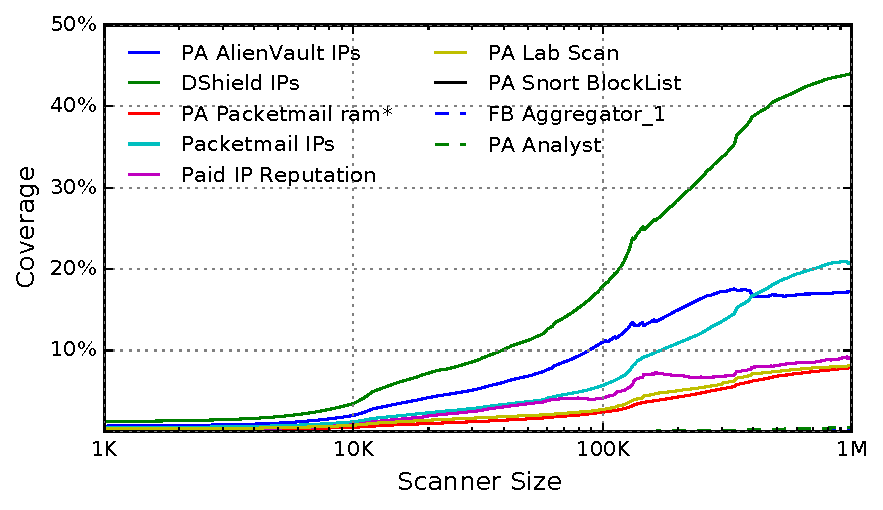
\includegraphics[width=0.8\textwidth]{data_character/images/caida_coverage_cdf.pdf}
\caption{The coverage of each feed on different sizes of scanners.}
\label{fig:caida_coverage_cdf}
\end{figure}

\finding\
The union of all the scan IPs in the feeds covers less than
2\% of the scanners collected by the telescope. Even if we only look
at the scanners with sizes larger than 10,000, the overall coverage is still
around 10\%, suggesting the coverage capability of scan feeds
is very limited. The graph shows that, as the scanner size increases, the coverage of
each feed over the datasets also increases, and large feeds cover more percent
of telescope scanners than small feeds. This trend aligns with the intuition that
scan feeds tend to capture more extensive scanners.

It is surprising that the small scan feeds in our collection have a smaller percentage of their
IPs shared with telescope scanners. This contradicts the idea that small feeds
would contain a larger percentage of extensive scanners (that would most likely also be observed by the telescope).

%Using another metric, the volume of scanners in the
%telescope is over 20 times larger than that of the scan feeds, yet the
%telescope scanners only cover 25.9\% of all of the scanning feeds'
%data. The overall volume of scanning activities is so extensive that
%even a /8 telescope will miss many of them, particularly if scanners
%are selective in targets (avoiding or focusing on certain IP ranges)
%or rate limits (falling below scanner labeling thresholds). The
%coverage curve based on scanner sizes showed that scan feeds are
%better at capturing large scanners, which is intuitive, but that a
%larger feed does not necessarily mean better coverage.


%\begin{table}
%\small
%\caption{Intersection between scan feeds and telescope scanners.
%\textit{Volume} contains the total amount of IPs in each feed from
%Jan. 2016 to July 2016. \textit{Intersection} is the proportion
%of each feed's IPs that overlap with the telescope data.}
%\centering
% \resizebox{0.7\linewidth}{!}{
%\begin{tabular}{l r r }
%\toprule
%Feed & Volume & Intersection \\
%\midrule
%{PA Snort BlockList}     & 312,533   & 18.2\% \\
%{\feedetiprep}           & 293,484   & 22.1\% \\
%{\feedpacketmail}        & 50,723    & 83.6\% \\
%{PA Packetmail ramnode}  & 11,452    & 76.1\% \\
%{\feedalienvault}        & 8,695     & 35.1\% \\
%{PA Malicious IPs}       & 7,960     & 63.3\% \\
%{PA Packetmail CARISIT}  & 5,955     & 71.5\%\\
%{PA SANS Top IPs}        & 3,087     & 77.4\%\\
%{PA Analyst}             & 444       & 52.0\%\\
%{PA Shockpot IPs}        & 156       & 50.0\%\\
%{PA SANS IPs}            & 129       & 63.6\%\\
%{FB Aggregator}          & 103       & 37.9\%\\
%\midrule
%Total & 675,243 & 25.9\%\\
%\bottomrule
%\end{tabular}
%}
%\label{tab:caida_ip_overlap}
%\end{table}




%\subsection{Inter-Category}
%
\textcolor{red}{TODO: Inter category analysis}

%Pick three or four categories of feeds, analyze their \textit{overlap}, \textit{uniquness} and \textit{time attributes}
%\label{sec:analysis}
%\input{content/analysis_scan.tex}

\section{File Hash Threat Intelligence}
\label{sec:hash-analysis}

File hashes in a threat intelligence feed are indicators for malicious
files. It is one of the most lightweight ways to mark files as
suspicious. One can incorporate this data to block malicious
downloads, malicious email attachments, and malware. Likewise, file
hashes can be used to whitelist applications and these feeds can be
used to ensure malicious files do not appear in a customer's
whitelist. In this section we present our analysis on
eight file hash feeds, also collected from December 1st, 2017
to July 20th, 2018. We use the same metrics defined in
Section~\ref{sec:metrics}.

The file hash feeds we collected use a range of different hash
functions to specify malicious files, including MD5, SHA1, SHA256 and
SHA512 (and some feeds provided values for multiple different hash
functions to support interoperability).  Since most indicators in our
dataset are MD5s, we have normalized to this representation by using other
feeds and the VirusTotal service to identify hash aliases for known
malicious files (i.e., which MD5 corresponds to a particualr SHA256
value).  


\begin{table*}[htt]
\footnotesize \tabcolsep=0.11cm
\caption{File hash feeds overview.
The second column group presents feed volume, average daily rate, the number of converted MD5s (Section~\ref{sec:hash-overlap}) and exclusive proportion.
\textit{Not in VT} is fraction of hashes that are not found in VirusTotal, \textit{Not det.} the fraction of hashes that are found in VirusTotal but are not labeled as malicious by any products, and \textit{Detected} the fraction that are found in VirusTotal and are labeled malicious by at least one product. Column \textit{Not in SD} shows the fraction of hashes in a feed that are not in Shadowserver Bin Check. \textit{In NSRL} and \textit{In AppInfo} show the absolute number of hashes found in Shadowserver (Section~\ref{sec:hash-accuracy}). \textit{Exclusive} is based on the MD5-normalized hashes counted under \textit{Converted}. All the other percentages in the table are based on \textit{Volume}.
}
\centering
\small
\begin{tabular}{l | r r r r| r r r | r r r }
\toprule
 Feed         &   Volume  &  Avg. Rate  & Converted &   Exclusive  &   Not in VT    &  Not det.  &   Detected   &   Not in SD &   In NSRL   &  In AppInfo  \\
\midrule
 FB Malware              &    944,257  &  4,070    & 944,257   &    >99.99\%    &     37.41\%    &    50.50\%      &     12.09\%          &    99.89\% &     442 &             706 \\
 PA Malware Indicators   &    39,702   &  171      & 39,702    &     98.73\%    &      0.02\%    &     0.04\%      &     99.94\%          &   >99.99\% &       2 &             0  \\
 PA Analyst              &    38,586   &  166      & 37,665    &     97.97\%    &      4.26\%    &     2.82\%      &     92.92\%          &    99.95\% &       8 &             19 \\
 PA Twitter Emotet       &    1,031    &  4.44     & 960       &     77.29\%    &     11.74\%    &     0.78\%      &     87.49\%          &    99.81\% &       0 &             2  \\
 PA OSINT                &    829      &  3.57     & 783       &     71.65\%    &     19.06\%    &     0.84\%      &     80.10\%          &    99.88\% &       1 &             0  \\
 PA Sandbox              &    298      &  1.28     & 115       &     95.65\%    &     72.81\%    &     0.34\%      &     26.85\%          &    100\% &         0 &             0  \\
 PA Abuse.ch             &    267      &  1.15     & 3         &       100\%    &     98.88\%    &     0.75\%      &      0.37\%          &    100\% &         0 &             0  \\
 PA Zeus Tracker         &    17       &  0.07     & 17        &       100\%    &     88.24\%    &     5.88\%      &      5.88\%          &    100\% &         0 &             0  \\
\bottomrule
\end{tabular}
\label{tab:md5-volume}
\end{table*}

\subsection{Volume}

File hashes, unlike IP threat data, are not transient---a file does
not change from malicious to benign---and thus a far simpler volume
analysis is appropriate. I report volume as the number of new hashes
that are added to each feed during the measurement period.

As seen in Table~\ref{tab:md5-volume-1}, I examine each feed's volume and
average daily rate. Like IP feeds, file hash feeds also vary dramatically in
volume. The majority of the hashes are concentrated in three feeds: FB Malware,
PA Malware Indicators, and PA Analyst, which also exhibit the highest daily rates.
The other feeds are multiple order of magnitude smaller comparatively.

%Every feed has mostly exclusive content, with the ``lowest'' exclusivity belonging to PA Twitter Emotet and PA OSINT (still 77.6\% and 79.29\%, respectively). All other feeds showcase a >97\% exclusive percentage, demonstrating that most MD5 feeds are distinct from each other.

\subsection{Intersection and Exclusive Contribution}
\label{sec:hash-overlap}

As we mentioned earlier, to conduct intersection and exclusive
analysis of file hash feeds, we need to convert indicators into the
same hash type. Here we convert non-MD5 hashes into MD5s, using either
metadata in the indicator itself (i.e., if it reports values for
multiple hash functions) or by querying the source hash from
VirusTotal~\cite{VirusTotal} which reports the full suite of hashes
for all files in its dataset.  However, for a small fraction of hashes
we are unable to find aliases to conver them to the MD5 representation
and must exclude them from the analysis in this section.  This filtering is
reflected in Table~\ref{tab:md5-volume}, in which the Volume column
represents the number of unique hashes found in each feed and the Converted
column is the subset that we have been able to normalize to a MD5
representation.

\finding\ The intersections between hash feeds are minimal,
even among the feeds that have multiple orders of magnitude differences in size.
Across all feeds, only PA Analyst has relatively high intersections: PA Analyst
shares 27\% of PA OSINT's MD5s and 13\% of PA Twitter Emotet's MD5s. PA Malware
Indicators has a small intersection also with these two feeds. All other
intersections are around or less than 1\%. Consequently, the vast majority of
MD5s are unique to one feed, as recorded in column \textit{Exclusive} in
Table~\ref{tab:md5-volume}. The ``lowest'' exclusivity belongs to PA Twitter
Emotet and PA OSINT (still 77.29\% and 71.65\%, respectively). All other feeds
showcase an over 95\% exclusive percentage, demonstrating that most file hash feeds
are distinct from each other.

Due to the different sources of malware between feeds, a low intersection is to
be expected in some cases. For example, PA Twitter Emotet and PA Zeus Tracker
should have no intersection, since they are tracking different malware strains.
The other, more general feeds could expect some overlap, but mostly exhibit
little to no intersection. Considering the sheer volume of the FB Malware feed,
one might expect it would encapsulate many of the smaller feeds or at least
parts of them. This is not the case, however, as FB Malware has a negligible
intersection with all other feeds.

Due to the lack of intersection among the feeds, we omit the latency analysis
of the hash feeds, as there is simply not enough intersecting data to conclude
which feeds perform better with regards to latency.

%\subsection{Latency}
\label{sec:hash-timing}
\note{We might need to delete this section since the overlapped parts are too small, we can't make an argument about latency}

We use the same relative latency definition to calculate the latency distribution of MD5s in each feed, and the calculation is based on the shared data between feeds. Since MD5s are not transient, we don't need to set a time restriction for this computation. Figure~\ref{fig:md5-latency} shows the latency distribution CDF of the feeds.

\begin{figure}[h]
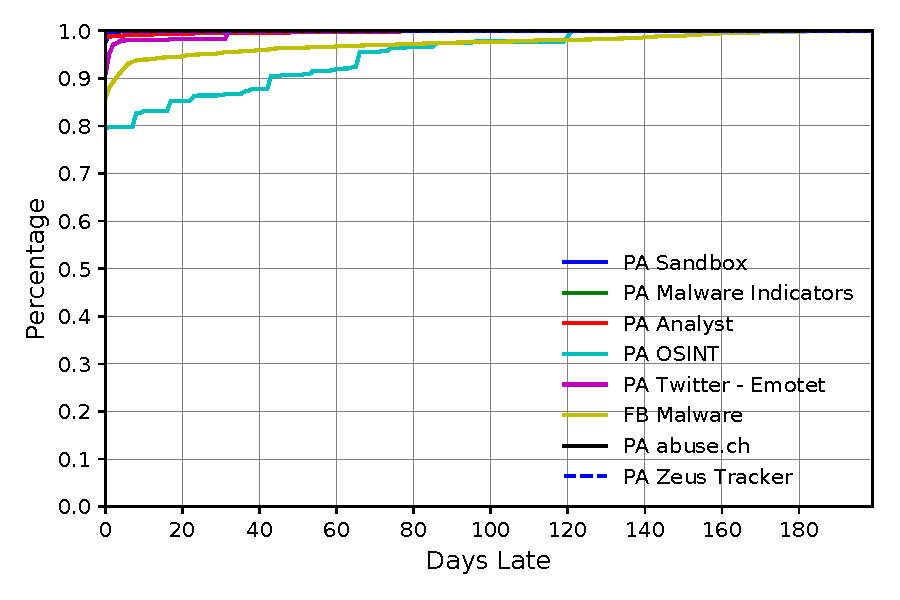
\includegraphics[width=0.9\columnwidth]{images/md5_lateDay.pdf}
\caption{Feed Latency Distribution showing what percentage of each feed's intersected samples are on a particular delay.}
\label{fig:md5-latency}
\end{figure}

As seen in Figure~\ref{fig:md5-latency}, the feeds are roughly grouped into 3 areas. {PA Malware Indicators}, {PA Zeus Tracker}, {PA Analyst}, {PA Twitter - Emotet}, {PA abuse.ch} and {PA Sandbox} report over 90\% of their data first, while {FB Malware }reports over 85\% of its data first. PA OSINT is the outlier in the graph which reports only 80\% of its shared data first. It also has the largest delays, taking almost 50 days to reach 90th percentile and over 70 days to reach 95th percentile.

\finding\ The latency analysis shows which feed is more effective from a timing standpoint, and again demonstrates the fact that a large \ti\ source is not always the quickest at reporting threats.

\subsection{Accuracy}
\label{sec:hash-accuracy}
Assessing the accuracy of file hash feeds presents a problem: there is no
universal ground truth to determine if a file is malicious or benign. Thus,
to gauge the accuracy of the feeds, we use two metrics: a check for malicious
hashes against VirusTotal, and a check for benign hashes against Shadowserver's
Bin Check service. Note that all the percentages discussed below are based on
the \textit{Volume} of each feed.

\subsubsection{VirusTotal}

VirusTotal is a service that is often used when analyzing
malware to get a base of information about a suspected file.
Anyone can upload a file to be scanned. Upon submission, these files will be
scanned by more than 70 antivirus scanners, which creates a report on how many
antivirus scanners mark it malicious, among other information. In this analysis,
we query VirusTotal for the hashes in each file hash feed and then inspect the
percent of hashes that are marked as malicious and how many AV scanners have
recorded them. Due to the high volume of the FB Malware feed and the query
rate limit of VirusTotal, we randomly sampled 80,000 hashes from the feed for
this analysis.

Table~\ref{tab:md5-volume} shows a breakdown of the base detection rates for
each feed from VirusTotal. As the PA feeds decrease in volume, the rates at
which they are found in VirusTotal also decreases. The larger PA feeds have a
much higher detection rate than their smaller counterparts. On the other hand,
FB Malware only has 37\% of its data detected by antivirus scanners and 50\% in
VirusTotal with no detection despite being the largest feed. This could indicate
that FB Malware focuses on threats that specifically target Facebook and that
are not as relevant to most VirusTotal users, such as malicious browser
extensions~\cite{dekoven2017malicious, jagpal2015trends, kapravelos2014hulk}.
This might undermine the limited coverage of VirusTotal as an oracle to detect
targeted threats that are not of broader interest.

\begin{figure}[t]
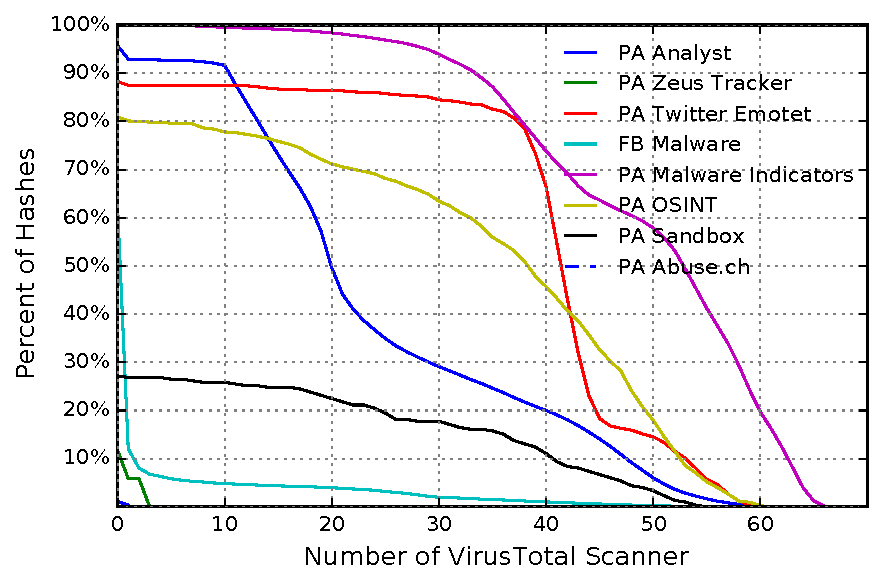
\includegraphics[width=0.95\columnwidth]{images/hash_vt_cdf.pdf}
\caption{VirusTotal detection distribution. Each point means the proportion of indicators (Y value) in a feed that is detected by \textit{over} X number of AV scanners in VirusTotal.}
\label{fig:vt-cdf}
\end{figure}

To further understand how the scanners in VirusTotal report the feed's data,
we plot a graph of what percentage of hashes in each feed are detected by how many
VirusTotal scanners. As seen in Figure~\ref{fig:vt-cdf}, four feeds have more
than 50\% of their samples detected by over 20 scanners. PA Malware Indicators
and PA Twitter Emotet did not experience a large detection drop before 35 scanners,
indicating that most indicators in the two feeds are popular malicious files
recognized by many AV vendors. While PA Sandbox has a large percent of its hashes
not presented in VirusTotal, over 70\% of its samples that are detected are marked
by over 20 AV scanners, showcasing a high confidence detection.

\subsubsection{Shadowserver}

To more fully gauge the accuracy of the file hash feeds,
we also examined how each feed measured against Shadowserver's Bin Check
Service~\cite{shadowserver}. The service checks file hashes against NIST's
National Software Registry List (NSRL) in addition to Shadowserver's own repository of
known software. Table~\ref{tab:md5-volume} details how each feed compares with
Shadowserver's Bin Check service.

It might be expected that there would be no hash found with Shadowserver's Bin
Check service, but it is not the case. Some of the samples from the feeds that
appear in Shadowserver are well known binaries such as versions of Microsoft
Office products, Window's Service Packs, calc.exe, etc. In the event malware
injects itself into a running process, it remains plausible that some of these
well-known binaries find their way into \ti\ feeds from users wrongly attributing
maliciousness. While FB Malware has over one thousand hashes in Shadowserver, this
is not a widespread issue, as all feeds have <1\% of their hashes contained within
Shadowserver's Bin Check service.
%, shown in Table \ref{tab:md5-volume}.
This showcases that while there are a few exceptions, the feeds mostly do not
contain well-known, benign files.

\finding\ Each PA feed has a negligible rate of occurrence within Shadowserver
regardless of their VirusTotal detection, showing they do not contain generic
false positives. Larger feeds exhibit high VirusTotal detection rates except
for FB Malware, while small feeds have relatively low detection rates.
This suggests that small hash feeds might focus more on specific malicious files
that are not widely known.
FB Malware has a low VirusTotal occurrence despite
its size and has over one thousand hashes in Shadowserver, but its overall low
percentage of hashes within Shadowserver indicates that it does not contain
many known files and might have threats not typically recognized by
VirusTotal's scanners.


\section{Longitudinal Comparison}
\label{sec:new_vs_old}

In addition to the measurement period considered so far (December 1, 2017 to July 20, 2018), I also analyzed data from the same IP feeds from January 1, 2016 to August 31, 2016. These two measurement periods, 23 months apart, allow us to measure how these IP feeds have changed in two years. Table~\ref{tab:old-volume-overview-1} and
Table~\ref{tab:old-volume-overview-2} summarizes the differences between these two measurement periods. \colname{Avg. Rate} shows the percentage of daily rate changed over the old feeds.
The two columns under \colname{Unrt} show the unroutable rates of feeds in 2016 and 2018 separately. The two columns under \colname{CDN} present the number of IPs fall in CDN IP ranges in old and new data. In the table, \colname{2018} represents the current measurement period and \colname{2016} the period  January 1, 2016 to August 31, 2016.
\newcolumntype{H}{>{\setbox0=\hbox\bgroup}c<{\egroup}@{}}

\begin{table}[t!]
\centering
\caption{Data changes in IP feeds compared against the ones in 2016, \colname{Avg. Rate} shows the percentage of daily rate changed over the old feeds.
The two columns under \colname{Unrt} show the unroutable rates of feeds in 2016 and 2018 separately. The two columns under \colname{CDN} present the number of IPs fall in CDN IP ranges in old and new data.}
\label{tab:old-volume-overview}
\scriptsize
 \begin{tabular}{l r H H H H H r r r r }
 \toprule
& & & & & & & \multicolumn{2}{c}{\colname{Unroutable}} & \multicolumn{2}{c}{\colname{CDN}} \\
\cmidrule(lr){8-9}\cmidrule(l){10-11}
 \colname{Feed} & \colname{Avg. Rate} & \colname{Exclusive} & \colname{Unrt} & \colname{Unrt} & \colname{CDNs} & \colname{New} &   2016 &  2018 &  2016  &  2018 \\ %& \colname{Unrt} \\
  \midrule
  \textbf{Scan Feeds} \\
  %\cline{1-1}
  PA AlienVault IPs 	    & $+$1,347\%    & 63.3\%  	& 18218.0  & +0.0        & +0     & 100\%   & 0.0\%    & 0.0\%      & 0    & 0 \\
  PA Packetmail ram* 	    & $+$733\%   & 75.3\% 	 	& 6749.8   & +0.0        & +0     & 100\%   & <0.01\%    & <0.01\%  	& 0    & 0 \\
  Packetmail IPs 	        & $+$135\%   & 83.4\% 	 	& 11145.8  & +0.0        & +0     & 99.4\%  & 0.0\%    & 0.0\%    	& 0     & 0\\
  Paid IP Reputation 	    & $-$57\%   & 97.7\% 	 	& 59430.9  & -7.08       & -889   & 91.3\%  & 8.73\%    & 1.65\%  & 910     & 21\\
  PA Lab Scan 	            & $-$1\%    & 85.1\% 	 	& 5921.8   & +<0.01      & +0     & 99.8\%  & 0.0\%     & <0.01\%   & 0   & 0 \\
  PA Snort BlockList 	    & $-$97\%   & 99.4\% 	 	& 123093.3 & +0.41       & -1     & 86.6\%  & <0.01\%     & 0.42\% 	& 1     & 0\\
  FB Aggregator$_1$ 	    & $+$332\%   & 83.8\% 	 	& 617.3    & +0.0        & -6     & 100\%   & 0.0\%     & 0.0\%     & 6   & 0 \\
  PA Analyst 	            & $-$44\%   & 52.5\% 	 	& 137.2    & +0.41       & +0     & >99.9\% & 0.0\%  	& 0.41\%    & 0   & 0\\

  %\midrule
  \textbf{Botnet Feeds} \\
  %\cline{1-1}
  PA CI Army 	            & $+$114\%   & 96.8\% 	& 4996.6  & +0.0     & +0    & 100\%  & <0.01\%  & <0.01\% & 0    & 0\\
  Paid IP Reputation 	    & $-$39\%   & 99.8\% 	& 17249.7 & +1.02    & +59   & 80.5\% & 0.63\%   & 1.66\%  & 15    & 74\\
  PA Botscout IPs 	        & $+$1\%    & 74.5\% 	& 5762.6  & +0.08    & -1    & 100\% & 0.01\%    & 0.09\%  & 1     & 0\\
  PA VoIP Blacklist 	    & $+$252\%   & 89.7\% 	& 732.4   & +0.32  	 & +0    & 100\% & 0.0\%     & 0.32\%  & 0    & 0\\
  PA Compromised IPs 	    & $-$36\%   & 94.9\% 	& 1515.8  & -0.10 	 & +0    & 100\% & 0.10\%    & 0.0\%   & 0   & 0\\
  PA Blocklist Bots 	    & $-$95\%	  & 82.0\% 	& 8282.6  & +0.0     & +0    & 100\% & 0.0\%     & 0.0\%   & 0    & 0 \\
  PA Project Honeypot 	    & $+$63\%	  & 48.3\% 	& 260.2   & +0.0     & +0    & 100\% & 0.0\%     & 0.0\%   & 0    & 0 \\

  %\midrule
  \textbf{Brute-force Feeds} \\
  %\cline{1-1}
   Badips SSH 	             & $+$30\%   & 94.2\% 	& 45479.9   & +0.12    & +1     & 97.6\% & 0.07\%      & 0.19\% & 0   & 1    \\
   Badips Badbots 	         & $+$1,732\%    & 87.6\%     & 1085.5    & +1.04    & +1064  & 92.6\% & 0.0\%      & 1.04\%  & 187 & 1,251   \\
   Paid IP Reputation 	     & $-$62\%   & 91.0\% 	& 19483.5   & -6.52    & -325   & 98.4\% & 6.55\%    & 0.03\%   & 335 & 10  \\
   PA Brute-Force 	         & $-$72\%   & 97.3\% 	& 63016.8   & +0.0     & +0     & 100\%  & 0.0\%      & 0.0\%   & 0   & 0  \\
   Badips Username*          & $+$3,040\%    & 16.6\% 	& 175.7     & +0.53    & +0     & 95.7\% & 0.0\%     & 0.53\% 	& 0  & 0\\
   Haley SSH 	             & $+$428\%   & 13.6\% 	& 226.6     & -0.01    & +0     & 94.8\% & 0.04\% 	& 0.03\%    & 0  & 0\\
   FB Aggregator$_2$ 	     & $+$387\%   & 42.4\% 	& 358.3     & -0.12    & +0     & 100\%  & 0.12\% 	& 0.0\%     & 0  & 0\\
   Nothink SSH 	             & $+$886\%   & 53.8\% 	& 778.5     & 0.95     & +0     & 86.4\% & 0.56\%	& 1.51\%    & 0  & 0\\
   Dangerrulez Brute 	     & $+$0\%	   & 9.15\% 	& 1109.8    & +0.0     & -1     & 99.8\% & 0.0\%    & 0.0\% 	& 1  & 0 \\

  %\midrule
  \textbf{Malware Feeds} \\
  %\cline{1-1}
  Paid IP Reputation 	       & $-$36\%	 & 96.2\% 	& 35273.7 	& -0.05     & -11,776   & 94.3\%& 0.18\%   & 0.13\% & 15265     & 3,489\\
  FB Malicious IPs 	           & $-$77\%   & 99.6\% 	& 17649.6   & -4.4      & -264      & 99.9\% & 6.81\%  & 2.14\% & 264     & 0   \\
  Feodo IP Blacklist 	       & $+$0\%    & 24.6\% 	& 589.0     & +0.0      & +0	    & 52.4\% & 0.0\%   & 0.0\% 	& 0      & 0 \\
  Malc0de IP Blacklist 	       & $-$9\%    & 60.0\%   & 143.1     & +0.0   	& -121      & 99.2\% & 0.0\%   & 0.0\%  & 132    & 11\\
  PA Bambenek C2 IPs 	       & $+$79\%   & 74.3\% 	& 72.9      & +9.13     & +0	    & 100\%  & 0.0\%   & 9.13\% & 0     & 0 \\
  PA SSL Malware IPs 	       & $-$34\%   & 30.1\% 	& 73.0      & +0.0      & +0	    & 100\%  & 0.0\%   & 0.0\%  & 0   & 0 \\
  PA Analyst 	               & $-$93\%    & 76.4\% 	& 917.7     & +0.0      & +0        & 99.8\% & 0.34\%  & 0.0\%  & 0  & 0\\
  PA Abuse.ch* 	               & $-$99\%   & 2.19\% 	& 4755.2    & +2.63     & +0        & 44.9\% & 0.49\%  & 3.12\% & 0  & 0\\
  PA Mal-Traffic-Anal  	       & $-$53\%   & 39.0\% 	& 25.7      & +0.51     & +0        & 100\%  & 0.0\%   & 0.51\%  & 0    & 0 \\
  Zeus IP Blacklist 	       & $-$66\%   & 24.3\%   & 164.8     & +0.0      & -6        & 49.2\% & 0.0\%   & 0.0\%   & 6  & 0\\


  %\midrule
  \textbf{Exploit Feeds} \\

Badips HTTP    & $+$326\%    & 98.0\% 	& 11693.1 	& +0.37  & +2,154  & 97.8\%   & 0.30\%  & 0.67\%  & 436 & 2,590 \\
Badips FTP 	   & $+$556\%    & 98.1\% 	& 6132.7    & +1.32  & +2      & 82.7\%   & 0.01\%  & 1.33\%  & 0   & 2\\
Badips DNS 	   & $+$9,525\%     & 96.9\% 	& 51.8      & +0.33  & +237    & 98.8\%   & 0.17\%  & 0.50\%  & 7   & 244  \\
Badips RFI 	   & $+$226\%    & 29.1\%  & 40.9      & +2.22  & -1      & 67.6\%   & 0.0\%   & 2.22\%  & 0   & 0  \\
%Badips SQL 	   & 66.6\% 	& 0.0 	& 0.0 \\

 \textbf{Spam Feeds} \\
  %\cline{1-1}
Paid IP Reputation 	 & $+$133\%	     & 99.9\%      & 4626.5    & +19.4   & +0      & 89.7\%  & 59.3\%    & 78.7\% & 0   & 0\\
Badips Spam 	     & $+$12,767\%    & 40.0\%      & 320.5     & +0.02   & +0      & 99.0\% 	& 0.0\%     & 0.02\% & 0   & 0 \\
Badips Postfix 	     & $-$53\%       & 99.1\%      & 52594.8   & +1.28   & +1      & 96.6\%  & <0.01\%   & 1.29\% & 0   & 1\\
PA Botscout IPs 	 & $+$18\%	     & 97.5\% 	  & 4337.3    & +0.06   & +0      & >99.9\%	& 0.0\%     & 0.06\% & 0   & 0 \\
AlienVault IP Rep 	 & $+$8\%	    & 87.2\% 	  & 1497.7    & -0.50   & +561    & 98.8\% 	& 0.57\%	& 0.07\% & 479  & 1,040 \\


\bottomrule
\end{tabular}
\end{table}



%\caption{Data changes in IP feeds compared against the ones in 2016, \colname{Avg. Rate} shows the change percentage of daily rate.
%For small changes we use ``\%'', for large changes we use ``x'', indicating x times.
%\colname{Unrt} shows the changes between unroutable rate with before. \colname{CDNs} are the changes on the number of IPs fail in into the CDN IP ranges.
%\colname{New} shows the percentage of indicators that are new to the recent feed compared with the old feed.}


\textbf{Volume.}
As shown in Table~\ref{tab:old-volume-overview-1} and ~\ref{tab:old-volume-overview-2}, feed volume has definitely changed after two years. Among 43 IP feeds that overlap both time periods,
21 have a higher daily rate compared with 2 years ago, 15 feeds
have a lower rate, and 7 feeds do not change substantially (the difference is below 20\%).
Volume can change dramatically over time, such as {\feedTSAlienVault}
in the scan category which is 13 times larger than before. On the other hand, a feed like {\feedTSBots} is now over 90\% smaller.

\textbf{Intersection and Exclusive Contribution.}
Despite the volume differences, the intersection statistics between feeds are largely the same across two years,
with feeds in scan and brute-force having high pairwise intersections and
feeds in other categories being mostly unique. Certain specific pairwise relations also did not change.
For example, {\feedbadipssh} still shared over 90\% of data in {\feeddangerrule} back in 2016, and {\feedetiprep} in malware
was still the only feed that has a non-trivial intersection with multiple small feeds.
Again, most data was exclusive to each feed two years ago: Across all
six categories more than 90\% of the indicators are not shared between feeds.

\textbf{Latency.}
The latency relationship between feeds was also similar:
timely feeds today were also timely two years ago, and the same with tardy feeds.
%The latency difference between feeds are bigger then compared with data, but small feeds
%still report a significant portion of their shared data.

\textbf{Accuracy.}
Feeds have more unroutable IPs now than before as shown in Table~\ref{tab:old-volume-overview-1} and~\ref{tab:old-volume-overview-2}:
In 2016, 22 of the 43 IP feeds had at least 1 unroutable IP; four feeds had unroutable rates over 1\%.
When checking the intersection with popular CDNs,
the feeds that contain IPs in CDN ranges two years ago are also the ones that have these IPs today.

\textbf{Shared indicators 2016--2018.}
I compared the data I collected from each feed in the two time periods, and found that 30
out of 43 feeds in 2018 intersect with their data from two years ago, and 9 feeds have
an intersection rate over 10\%. Three feeds in malware category, namely {\feedfeodo},
{\feedTSAbusech} and {\feedzeus}, have over 40\% of their data shared with the past feed,
meaning a large percent of C\&C indicators two years ago are still
identified by the feeds as threats today. Feeds in the botnet category, however, are very distinct from the
past, with all feeds having no intersection with the past except {\feedetiprep}.
\section{Absolute Latency}
\label{sec:abs_latency}

I defined the latency metric in this chapter as relative latency between \ti\
sources, since it is easy to compute and allows consumers to compare feeds
to each other on this aspect. However, it is also critical to know
about the absolute latency distribution of indicators. Absolute latency
represents how fast a feed can actually report a threat, which directly decides
the effectiveness of the data when used in a pro-active way. As I already
discussed in Section~\ref{sec:ip-timing}, absolute latency is hard to measure,
as I do not have ground truth of the underlying threat.

In Section~\ref{sec:completeness}, I used an Internet telescope as the approximation
for ground truth to measure the coverage of scan feeds. In Section~\ref{sec:hash-accuracy},
I used VirusTotal as an oracle to measure the accuracy of file hash feeds.
Although these sources are not real ground truth and it is unclear how far away
they are, these large and well-managed sources can help us, to a certain extent,
profile the performance of \ti\ feeds. In this section, I use these two sources
again to approximate the absolute latency of indicators in scan IP feeds and
malicious file hash feeds.

More specifically, I measure the latency of IPs in scan feeds
relative to the first occurrence time of the same IP in the scanners collected from
the telescope. Considering the massive size of the telescope, it should presumably
detect scanners much sooner after the scanning event actually happened.
I measure latency of file hashes relative to the \texttt{first\_seen} timestamps queried
from VirusTotal. The \texttt{first\_seen} timestamp represents the time when the corresponding
file is first uploaded to VirusTotal. VirusTotal is a very popular service and it is a
convention for many security experts to upload new malware samples to VirusTotal once
they discovered them. Therefore, this timestamp roughly entails when the security
community first noticed the malicious file and can be a good approximation for absolute
latency.

\begin{figure}[t!]
\centering
\subfloat[Latency distribution in scan feeds relative to the Internet telescope]{
	\label{fig:scan_abs_firstseen}
	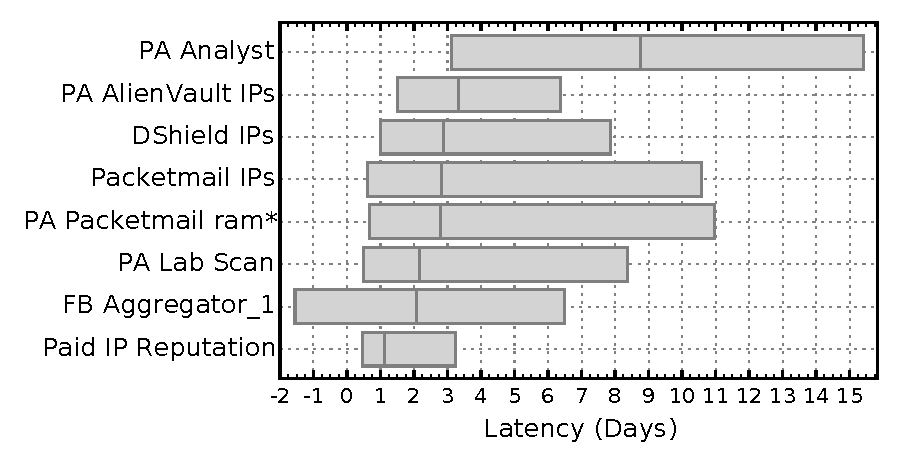
\includegraphics[width=0.8\textwidth]{data_character/images/scan_abs_latency.pdf}}

\subfloat[Latency distribution in file hash feeds relative to VirusTotal]{
	\label{fig:hash_abs_firstseen}
	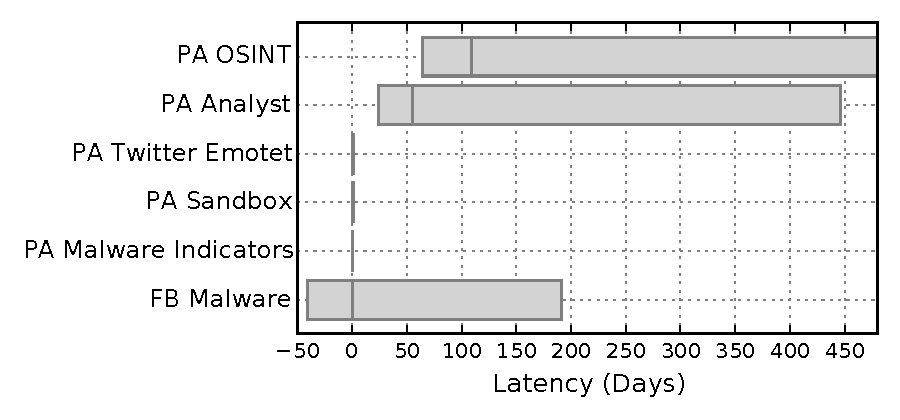
\includegraphics[width=0.8\textwidth]{data_character/images/hash_abs_latency.pdf}}

\caption{Distribution of indicators' latency in scan and file hash feeds.
The scan feeds' distribution are calculated in hour granularity while
the file hash feeds' distribution are calculated in day granularity.}
\label{fig:abs_firstseen}
\end{figure}


Figure~\ref{fig:abs_firstseen} show the latency distribution of each feed, using
the same plotting convention as in Section~\ref{sec:ip-timing}. Some feeds are not
shown in the figure as there are too little data points in those feeds to reason
about distribution.

\finding\
Comparing Figure~\ref{fig:scan_abs_firstseen} to Figure~\ref{fig:scan_firstseen},
I can see that the median latency of feeds are all larger. This is consistent with
my assumption that a large sensor tends to receive indiscriminate scanners sooner.
Scan feeds' median lantecy are one to three days relative to the Internet telescope,
except {\feedTSAnalyst}, whose median latency is almost nine days.
The order of median latency between feeds changed compared with Figure~\ref{fig:scan_firstseen},
but since the original relative median latencies among scan feeds are very close,
the new order here is more likely to be statistics variances. Also, note that
although the {\feedTSAlienVault} seems much slower than it is in
Figure~\ref{fig:scan_firstseen}, its 75 percentile latency is still the second
smallest one.

On the other hand, the latency distributions of hash feeds vary more dramatically.
PA Malware Indicators, PA Sandbox and PA Twitter Emotet are almost as fast as
VirusTotal: all three feeds have 25 percentile and median latency equal to zero.
PA OSINT and PA Analyst are comparatively much slower, and PA OSINT even has a 75
percentile latency of 1680 days. This might be because of the heterogeneous nature of
malware feeds. The figure also shows that feed volumes do not imply
their latency, as PA Analyst and FB Malware are much slower than the small hash
feeds.

Figure~\ref{fig:abs_firstseen} demonstrates that the Internet telescope and VirusTotal
are indeed good approximations for absolute latency measurement, as most
indicators in \ti\ feeds are observed relatively later. However, every scan
feed has over 2\% of its indicators detected earlier than the telescope did.
{\feedFBBasecamp} and {\feeddshield} even have over 10\% of their indicators observed
earlier. There is also a similar case in file hash feeds. This aligns with
my observation in Section~\ref{sec:ip-timing} that small feeds can still report
a non-trivial amount of their data first. Another interesting observation is that
both Facebook feeds, {\feedFBBasecamp} and FB Malware, have a large percent of
their data observed earlier than the telescope or VirusTotal. This again suggests
that Facebook (and its threat intelligence partners) might face more targeted
threats, so those threats will be first observed by Facebook.

\section{Discussion}
\label{sec:discussion}

\subsection{Metrics Usage}
Threat intelligence has many different potential uses. For example,
analysts may consume threat data interactively during manual
incident investigations, or may use it to automate the detection of
suspicious activity and/or blacklisting.  When not itself
determinative, such information may also be used to \emph{enrich}
other data sources, informing investigations or aiding in automatic
algorithmic interventions. We have introduced a set of basic threat
intelligence metrics---volume, intersection, unique contribution,
latency, coverage and accuracy---that can inform and quantify each of
those uses.  Depending on a number of factors, such as the intended
use case and the cost of false positives and negatives, some of
these metrics will become more or less important when evaluating a
\ti\ source. For example, a feed with poor accuracy but
high coverage might be ideal when an analyst is using a \ti\ source
interactively during manually incident investigations (since in this
case, the analyst, as a domain expert, can provide additional filtering
of false positives). Similarly, latency might not be a critical metric
in a retrospective use case (e.g., post-discovery breach
investigation).  However, if an organization is looking for a
\ti\ source where the IPs are intended to be added to a firewall's
blacklist then accuracy and latency should likely be weighted over
coverage, assuming that blocking benign activity is more costly.

Another common real-world scenario is that a company has a limited
budget to purchase \ti\ sources and has a specific set of threats (\ie
botnet, brute-force) they are focused on mitigating. In such cases,
the metrics we have described can be used directly in evaluating \ti\
options, biasing twoards sources that maximize coverage of the most
relevant threats while limiting intersection.


\subsection{Data Labeling}
Threat intelligence IP data carries different meanings. To properly use this
data, it is critical to know what the indicators actually mean: whether
they are Internet scanners, members of a botnet or malicious actors who
had attacked other places before. We have attempted to group feeds by their
intended meaning in our analysis.

However, this category information, which primarily comes from \ti\ sources
themselves, is not always available. Feeds such as {\feedalienvault} and
Facebook Threat Exchange sources contain a significant number
of indicators labeled ``Malicious'' or ``Suspicious.'' The meanings of
these indicators are unclear, making it difficult for consumers to decide
how to use the data and the possible consequences.

For feeds that provide category information, it is sometimes too broad
to be meaningful. For example, multiple feeds in our collection
simply label their indicators as ``Scanner.'' Network scanning can
represent port scanning (by sending SYN packets), or a vulnerability scan (by
probing host for known vulnerabilities). The ambiguity here, as a result of
ad-hoc data labeling, again poses challenges for security experts when using
\ti\ data.

Recently, standard \ti\ formats have been proposed and developed, notably
IODEF~\cite{IODEF}, CybOX~\cite{CybOX} and STIX~\cite{STIX}, that try to
standardize the threat intelligence presentation and sharing. But these
standards focus largely on the data format. There is room
to improve these standards by designing a standard \emph{semantics} for threat
intelligence data.

%Even if we just use it to block traffic, it is very difficult to justify the
%performance of this feed, let alone to use it during a threat forensic analysis.

% wrong categorization.
%Sometimes the categorization provided by the provider might not be acurrate. For example, the
%\feedTSSnort\ is labelled as scanners by the PA, however, we found little intersection between
%this source and other scan sources, also little intersectio with the scanners collected
%by the Internet telescope. We suspect the data provided by this feed is not real Internet scanners.

\subsection{Limitations}
There are several questions that our study does not address. We attempted to collect data from a diverse set of
sources, including public feeds, commercial feeds and industrial exchange feeds,
but it is inherently not comprehensive. There are some prohibitively expensive or
publication-restricted data sources that are not available to us. More specialized measurement
work should be done in the future to further analyze the performance of these
expensive and exclusive data sources.

%Future work might be to obtain access to a larger more diverse set of \ti\
%sources or incentives \ti\ providers to allow a neutral third-party to
%replicate our metrics.

A second limitation is our visibility into how different companies use threat
intelligence operationally. For a company, perhaps the most useful kind of metric
measures how a threat intelligence source affects its main performance indicators
as well as its exposure to risk. Such metrics would require a deep integration
into security workflows at enterprises to measure the operation effect of decisions
made using threat intelligence. This would allow CIOs and CSOs to better understand
exactly what a particular threat intelligence product contributes to a company. As
researchers, we do not use \ti\ operationally. A better understanding of operational
needs would help refine our metrics to maximize their utility for operations-driven consumers.

The third limitation is the lack of ground truth, a limitation shared
by all the similar measurement work. It is simply very difficult to obtain the full picture
of a certain category of threat, making it very challenging to precisely determine accuracy and coverage of feeds. In this
study, we used data from an Internet telescope and VirusTotal as a close approximation.
There are also a handful of cases where a security incident has been comprehensively studied by
researchers, such as the Mirai study~\cite{antonakakis2017understanding}, and such efforts
can be used to evaluate certain types of \ti\ data. But such studies are few in number.
One alternative is to try to establish the ground truth for a specific network.
For example, a company can record all the network traffic going in and out of its own network,
and identify security incidents either through its IDS system or manual forensic analysis.
Then it can evaluate the accuracy and coverage of a \ti\ feed under the context of its
own network. This can provide a customized view of \ti\ feeds.


%Our metrics can be used as a starting point and refined as needed based on an
%improved understanding of how \ti\ is currently used operationally and metrics
%that might improve the quality of \ti\ so that it could be used for additional tasks.


%%
%% Below are comments
%%
\begin{comment}
\subsection{Independence between Metrics}
We evaluated a large range of \ti\ sources using six metrics, it is
interesting to see if there is any correlation between these metrics.
We already compared the relation of between volume and latency of IP feeds
in Section~\ref{sec:ip-timing} and showed that there is not a strong correlation. Similar cases
can also be observed, for example, between volume and accuracy that neither high or low
volume implies high accuracy in our feeds collection. Also, both IP and MD5 feeds show
that the exclusive rate is irrelevant with the feeds' size.

To formally address this question, we check the correlation coefficient between
\emph{Volume}, \emph{Exclusive Contribution}, \emph{Latency} and \emph{Accuracy}
in IP and MD5 feeds(when available). The result shows a low(below 0.5) correlation across all comparison.
This means when choosing between different \ti\ sources, we need to evaluate them comprehensively
on multiple perspectives, as different perspective does not imply each other.

Coverage correlate with volume in our scan feeds, which is not a surprise since volume naturally
implies coverage when the accuracy are close.


\subsection{Limited Coverage}
Most \ti\ indicators are exclusive to each feed, for both IP and MD5 sources.
Moreover, when comparing with broad sensor data in known categories like Internet scanning,
fewer than 2\% of ``known bad'' addresses appear in all the data sources we
analyzed. These suggest several non-exclusive possibilities. First is that the
underlying space of indicators (both IP addresses and malicious file hashes) is
large and each individual data sources can at best sample a small fraction
thereof. Second, different measurement methodologies---even for the same threat
category---will select for different sub distributions of the
underlying ``ground truth'' data.  Third, this last effect is likely
exacerbated by the fact that not all threats are experienced uniformly
across the Internet and thus, some kinds of methodologies, will skew
to either favor or disfavor targeted attacks.

This implies that \ti\ consumers should focus more on how the feeds related to the
specific threat that the consumers are mostly exposed to, instead of blindly trying to maximize
coverage or to find the ``best'' feed. Future work would be to correlate \ti\ feeds' data
with the companies or organizations' network traffic and evaluate feeds under specific environments.
\end{comment}

%\section{Related Work}
\label{sec:background}

Several studies have examined the effectiveness of blacklist-based threat
intelligence~\cite{kuhrer2014paint, ramachandran2006revealing, ramachandran2007filtering, sheng2009empirical, sinha2008shades}.
Ramachandran~\etal~\cite{ramachandran2007filtering} showed that spam blacklists
are both incomplete (missing 35\% of the source IPs of spam emails captured in
two spam traps), and slow in responding (20\% of the spammers remain unlisted
after 30 days). Sinha~\etal~\cite{sinha2008shades} further confirmed this
result by showing that four major spam blacklists have very high false negative
rates, and analyzed the possible causes of the low coverage.
Sheng~\etal~\cite{sheng2009empirical} studied the effectiveness of
phishing blacklists, showing the lists are slow in reacting to
highly transient phishing campaigns. These studies focused on specific
types of threat intelligence sources, and only evaluated their operational
performance rather than producing empirical evaluation metrics for
threat intelligence data sources.

Other studies have analyzed the general attributes of threat
intelligence data.  Pitsillidis~\etal~\cite{tasters:imc12} studied the
characteristics of spam domain feeds, showing different perspectives
of spam feeds, and demonstrated that different feeds are suitable for
answering different questions.  Thomas~\etal~\cite{thomas2016abuse}
constructed their own threat intelligence by aggregating the abuse
traffic received from six Google services, showing a lack of
intersection and correlation among these different sources.  While
focusing on broader threat intelligence uses, these studies did not
focus on generalizable threat metrics that can be extended beyond the work.

Little work exists that defines a general measurement methodology to
examine threat intelligence across a broad set of types and categories.
Metcalf~\etal~\cite{metcalf2015blacklist} collected and measured IP
and domain blacklists from multiple sources, but only focused on volume
and intersection analysis. In contrast, we formally define a set of threat intelligence
metrics and conduct a broad and comprehensive study over a rich variety of
threat intelligence data. We conducted our measurement from the
perspective of consumers of \ti\ data
to offer guidance on choosing between different sources.
Our study also demonstrated the limitation of threat intelligence more thoroughly,
providing comprehensive characteristics of cyber threat intelligence that no work had
addressed previously.

%\section{Conclusion}
\label{sec:conclusion}

This paper has focused on the simplest, yet fundamental, metrics about
threat intelligence data. Using the proposed metrics, we measured a broad
set of \ti\ sources, and reported the characteristics and limitations of
\ti\ data. In addition to the individual findings mentioned in each section, here
we highlight the high-level lessons we learned from our study:

%---effectively investigating the extent to which disparate
%sources are measuring the same underlying empirical phenomena and can
%be meaningfully used to directly anticipate future attacks.  Thus far
%the evidence for this goal is spartan at best.

\begin{itemize}
	\item \ti\ feeds, far from containing
    homogeneous samples of some underlying truth, vary tremendously in the
    kinds of data they capture based on the particularities of their
    collection approach. Unfortunately, few \ti\ vendors explain the
    mechanism and methodology by which their data are collected and thus
    \ti\ consumers must make do with simple labels such as
    ``scan'' or ``botnet'', coupled with inferences about the
    likely mode of collection. Worse, a significant amount of data does not
    even have a clear definition of category, and is only labelled as
    ``malicious'' or ``suspicious'', leaving the ambiguity to consumers to
    decide what action should be taken based on the data.

    \item There is little evidence
    that larger feeds contain better data, or even that there are
    crisp quality distinctions between feeds across different categories
    or metrics (i.e., that a \ti\ provider whose feed performs well on one
    metric will perform well on another, or that these rankings will hold
    across threat categories). How data is collected also does not
    necessarily imply the feeds' attributes. For example, crowdsourcing-based feeds (\eg\ Badips feeds), are not always slower in reporting data
    than the self-collecting feeds (like \feedetiprep).

    \item Most IP-based \ti\ data sources are collections of
    singletons (i.e., that each IP address appears in at most one source)
    and even the higher-correlating data sources frequently have
    intersection rates of only 10\%. Moreover, when comparing with broad
    sensor data in known categories with broad effect (e.g., random
    scanning) fewer than 2\% of observed scanner addresses appear in most of
    the data sources we analyzed; indeed, even when focused on the largest
    and most prolific scanners, coverage is still limited to 10\%. There
    are similar results for file hash-based sources with little overlap
    among them.
\end{itemize}

The low intersection and coverage of \ti\ feeds could be the result of
%Taken together these suggest
several non-exclusive possibilities.
First is that the underlying space of indicators (both IP addresses
and malicious file hashes) is large and each individual data source
can at best sample a small fraction thereof.  It is almost certain
that this is true to some extent.  Second, different collection
methodologies---even for the same threat category---will select for
different sub distributions of the underlying ground truth data.
Third, this last effect is likely exacerbated by the fact that not all
threats are experienced uniformly across the Internet and, thus,
different methodologies will skew to either favor or disfavor targeted
attacks.


\begin{comment}
While resolving this question is of academic interest, it seems clear
that blindly using \ti\ data---even if one could afford to acquire
many such sources---is unlikely to be effective.  Proactive defenses,
such as blocking network connections or file executions that match
\ti\ indicators, are predicated on knowing, in advance, a large
fraction of the universe of future indicators; the evidence is that
this is not currently possible.  While there may be some utility in
doing this even for the small percentage of malicious traffic that may
be identified, this must be balanced against the costs of obtaining
and managing \ti\ data as well as the risks associated with false
positives.
\end{comment}


Based on our experience analyzing \ti\ data, we try to provide several
recommendations for the security community on this topic moving forward:

\begin{itemize}
    \item The threat intelligence community should standardize data labeling,
    with a clear definition of what the data means and how the data is collected. Security experts can then assess
    whether the data fit their need and the type of action should be taken
    on this data.

    \item There are few rules of thumb in selecting among \ti\ feeds,
    as there is not a clear correlation between different feed properties.
    Consumers need empirical metrics, such as those we describe, to
    meaningfully differentiate data sources, and to prioritize certain metrics
    based on their specific need.

    \item Blindly using \ti\ data---even if one could afford to acquire
    many such sources---is unlikely to provide better coverage and is
    also prone to collateral damage caused by false positives. Customers
    need to be always aware of these issues when deciding what action
    should be taken on this data.

    \item Besides focusing on the \ti\ data itself, future work should investigate
    the operational uses of threat intelligence in industry, as
    the true value of \ti\ data can only be understood in operational scenarios.
    Moreover, the community should explore more potential ways of using the data,
    which will extend our understanding of threat intelligence and also influence
    how vendors are curating the data and providing the services.

\end{itemize}


%However, this is only one potential use of threat intelligence data.
There are many ways we can use threat intelligence data.
It can be used to \emph{enrich} other information
(e.g., for investigating potential explanations of a security
incident), as a probabilistic canary (i.e., identifying an overall
site vulnerability via a single matching indicator may have value even
if other attacks of the same kind are not detected) or in providing a
useful source of ground truth data for supervised machine learning
systems. However, even given
such diverse purposes, organizations still need some way to prioritize which
\ti\ sources to invest in.  Our metrics provide some direction for
such choices. For example, an analyst who expects to use \ti\ interactively
during incident response would be better served by feeds with higher coverage,
but can accommodate poor accuracy, while an organization trying to
automatically label malicious instances for training purposes (e.g.,
brute force attacks) will be better served by the converse.  Thus, if
there is hope for demonstrating that threat intelligence can
materially impact operational security practices, we believe it will
be found in these more complex uses cases and that is where future
research will be most productive.
